% ==========
% CHƯƠNG 7
% ==========
\OpenGrid

\ParallelChapter
  {Reasoning with Geometry}
  {Luận với hình học}
  {}

\TriPara
  {
    \EN{Classically, geometry has been the subject in which students encounter mathematical proof based on formal deduction. Although proof should be naturally incorporated in all areas of the curriculum, attention to proof in the geometry curriculum is strengthened by a focus on reasoning and sense making. In addition, geometry has connections with other mathematical domains and important applications in careers and in everyday life. Geometric ideas are a significant part of many high-technology developments, including high-definition television (HDTV), global positioning systems (GPS), computer animation, computerized axial tomography (CAT) scans, cellular telephone networks, robotics, virtual reality, and docking of the Space Shuttle. Geometric and visual reasoning often enter our daily lives.}
  }
  {
    \VI{Theo truyền thống, hình học là môn học trong đó học sinh tiếp xúc với chứng minh toán học dựa trên suy diễn hình thức. Mặc dù chứng minh cần được tích hợp tự nhiên trong mọi mảng của chương trình học, việc chú trọng chứng minh trong chương trình hình học được củng cố nhờ trọng tâm đặt vào luận và hiểu. Bên cạnh đó, hình học có mối liên hệ với những lĩnh vực toán học khác và có ứng dụng quan trọng trong nghề nghiệp cũng như trong đời sống hằng ngày. Các ý tưởng hình học giữ vai trò quan trọng trong nhiều phát triển công nghệ cao, bao gồm truyền hình độ phân giải cao (HDTV), hệ thống định vị toàn cầu (GPS), hoạt hình máy tính, chụp cắt lớp vi tính (CAT), mạng điện thoại di động, robot, thực tế ảo và hoạt động ghép nối của tàu con thoi không gian. Luận hình học và luận trực quan thường hiện diện trong đời sống hằng ngày.}
  }
  {
    \NOTE{Cụm \emph{suy diễn hình thức} trong đoạn này cần được hiểu như một đơn vị nghĩa hoàn chỉnh. Trước hết, \emph{suy diễn} chỉ cách đi tới kết luận từ những điều đã được chấp nhận trước, chẳng hạn giả thiết, định nghĩa, tiên đề hoặc các kết quả đã biết. Ở đây, kết luận không được hình thành bằng cách thử nhiều trường hợp rồi đoán ra quy luật, mà bằng cách lần theo những hệ quả được rút ra từ cái đã có. Tiếp đó, từ \emph{hình thức} nhấn mạnh rằng các bước suy ra ấy phải được trình bày đủ rõ để có thể kiểm tra tính hợp lệ của từng bước. Vì vậy, \emph{suy diễn hình thức} không chỉ là suy ra một kết luận, mà là suy ra nó bằng một chuỗi bước minh bạch, chặt chẽ, và có thể biện minh được. Hiểu như vậy sẽ thấy vì sao hình học, theo truyền thống, thường là nơi học sinh gặp chứng minh toán học dựa trên suy diễn hình thức. Trong hình học, từ giả thiết của bài toán, học sinh phải dùng định nghĩa, tính chất và định lí để đi dần tới kết luận; chính quá trình ấy làm lộ rõ bản chất của chứng minh như một chuỗi bước suy ra có cơ sở. Cũng cần phân biệt \emph{suy diễn} với \emph{quy nạp}. Ở nghĩa rộng, suy diễn đi từ điều đã biết hoặc đã giả định tới kết luận, còn quy nạp đi từ những trường hợp riêng, những quan sát hay mẫu hình để hình thành một phỏng đoán tổng quát hơn. Theo nghĩa ấy, chúng là hai hướng vận động khác nhau của luận. Tuy nhiên, ở đây không nên đặt \emph{quy nạp toán học} cạnh \emph{suy diễn hình thức} như thể đó là một cặp đối xứng. Lí do là \emph{quy nạp toán học}, mặc dù mang chữ ``quy nạp'', lại là tên của một phương pháp chứng minh chặt chẽ; về vị thế toán học, nó thuộc phía chứng minh hình thức chứ không thuộc phía quy nạp theo nghĩa đi từ trường hợp riêng tới phỏng đoán.}
  }

\TriPara
  {
    \EN{A considerable amount of research on students' thinking in geometry can be used to promote students' reasoning and sense making in this area. Much of this research bolsters the van Hiele levels of students' geometric thinking (Battista 2007). These five van Hiele levels of thinking are sequential and hierarchical, meaning that students must pass through lower levels if they are to attain higher levels. The van Hiele levels of students' thinking can be linked to the reasoning habits described in chapter 2 and can help promote students' attainment of the reasoning and sense-making abilities exemplified in this publication. For instance, the first two van Hiele levels, \emph{visual-holistic} and \emph{descriptive-analytic} reasoning, link to the \emph{empirical} reasoning level described in ``Progression of Reasoning'' in chapter 2. The third van Hiele level, \emph{relational-inferential} reasoning, connects with the \emph{preformal} level, and the fourth and fifth van Hiele levels, \emph{formal deductive proof} and \emph{rigor}, are tied to the \emph{formal} level of reasoning. Accordingly, knowledge about students' thinking not only allows us but requires us to support students at whatever level of thinking they may have attained when coming to high school and to provide them experiences that help them move to higher levels.}
  }
  {
    \VI{Nhiều nghiên cứu về tư duy hình học của học sinh có thể được dùng để thúc đẩy luận và hiểu của học sinh trong mảng này. Phần lớn nghiên cứu ấy củng cố cơ sở cho các mức tư duy hình học của học sinh theo van Hiele (Battista 2007). Năm mức tư duy theo van Hiele này có tính tuần tự và thứ bậc, nghĩa là học sinh phải đi qua các mức thấp hơn nếu muốn đạt tới các mức cao hơn. Các mức tư duy của học sinh theo van Hiele có thể được liên kết với những thói quen luận được mô tả trong Chương 2, và có thể góp phần thúc đẩy việc học sinh đạt tới các năng lực luận và hiểu được minh họa trong công trình này. Chẳng hạn, hai mức đầu tiên theo van Hiele, \emph{luận trực quan--toàn thể} và \emph{luận mô tả--phân tích}, liên kết với mức luận \emph{thực nghiệm} được mô tả trong mục ``Tiến trình phát triển của luận'' ở Chương 2. Mức thứ ba theo van Hiele, \emph{luận quan hệ--suy luận}, tương ứng với mức \emph{tiền hình thức}, còn mức thứ tư và thứ năm, \emph{chứng minh suy diễn hình thức} và \emph{nghiêm ngặt}, gắn với mức luận \emph{hình thức}. Vì thế, hiểu biết về tư duy của học sinh không chỉ cho phép mà còn buộc người dạy phải hỗ trợ học sinh ở bất cứ mức tư duy nào các em đã đạt tới khi bước vào trung học phổ thông, đồng thời tạo cho các em những trải nghiệm giúp các em chuyển lên mức cao hơn.}
  }
  {
    \NOTE{Đoạn này đưa cơ sở nghiên cứu về tư duy hình học của học sinh vào trung tâm của định hướng dạy học. Điều tác giả muốn nhấn mạnh không chỉ là sự tồn tại của mô hình van Hiele, mà là hệ quả sư phạm của nó: sự phát triển tư duy hình học có tính tuần tự và thứ bậc, nên không thể đòi hỏi học sinh đạt tới chứng minh hình thức khi các em còn chưa đi qua những mức tư duy thấp hơn. Vì thế, nghiên cứu về tư duy của học sinh không phải một tri thức phụ trợ đứng ngoài lớp học, mà là căn cứ để quyết định nên yêu cầu gì và nên nâng đỡ học sinh theo hướng nào.

    Điểm quan trọng hơn nữa là tác giả không dùng van Hiele như một lí thuyết riêng của hình học, tách biệt khỏi phần còn lại của cuốn sách. Các mức van Hiele được nối trực tiếp với tiến trình phát triển của luận đã trình bày ở Chương 2: hai mức đầu gắn với luận thực nghiệm, khi học sinh còn dựa nhiều vào quan sát và mô tả; mức thứ ba tương ứng với giai đoạn tiền hình thức, khi các quan hệ và suy ra bắt đầu hiện rõ; hai mức cao nhất gắn với luận hình thức, nơi chứng minh và tính chặt chẽ trở thành trung tâm. Nhờ cách nối này, hình học không hiện ra như một ngoại lệ trong sách, mà như một miền trong đó cùng một tiến trình phát triển của luận và hiểu được biểu hiện dưới một dạng đặc thù.

    Câu kết của đoạn văn mang ý nghĩa sư phạm quyết định. Hiểu biết về tư duy của học sinh không chỉ cho phép mà còn buộc người dạy phải bắt đầu từ mức độ mà học sinh thực sự đang có, rồi tổ chức những trải nghiệm thích hợp để các em từng bước đi lên. Ở đây, tác giả đang bác bỏ ngầm một cách dạy quen thuộc: đòi hỏi quá sớm những hình thức suy diễn mà học sinh chưa có nền nhận thức để mang nổi. Đồng thời, đoạn này cũng biện minh cho giá trị của các hoạt động trực quan, mô tả và khám phá như những chặng cần thiết trên con đường đi tới chứng minh hình thức.}
  }

\TriPara
  {
    \EN{Key elements of reasoning and sense making with geometry include the following:

    \begin{itemize}
      \item \emph{Conjecturing about geometric objects.} Analyzing configurations and reasoning inductively about relationships to formulate conjectures.
      
      \item \emph{Construction and evaluation of geometric arguments.} Developing and evaluating deductive arguments (both formal and informal) about figures and their properties that help make sense of geometric situations.
      
      \item \emph{Multiple geometric approaches.} Analyzing mathematical situations by using transformations, synthetic approaches, and coordinate systems.
      
      \item \emph{Geometric connections and modeling.} Using geometric ideas, including spatial visualization, in other areas of mathematics, other disciplines, and in real-world situations.
    \end{itemize}

    We address these key elements in more detail in the following sections.}
  }
  {
    \VI{Các yếu tố then chốt của luận và hiểu với hình học gồm có:

    \begin{itemize}
      \item \emph{Phỏng đoán về các đối tượng hình học.} Phân tích cấu hình hình học và luận theo hướng quy nạp về các quan hệ để hình thành phỏng đoán.
      
      \item \emph{Xây dựng và thẩm định các lập luận hình học.} Phát triển và thẩm định các lập luận suy diễn (cả hình thức lẫn phi hình thức) về các hình và tính chất của chúng nhằm giúp hiểu các tình huống hình học.
      
      \item \emph{Nhiều cách tiếp cận hình học.} Phân tích tình huống toán học bằng cách sử dụng phép biến hình, cách tiếp cận tổng hợp, và hệ tọa độ.\vspace{\baselineskip}
      
      \item \emph{Các kết nối hình học và mô hình hóa.} Sử dụng ý tưởng hình học, bao gồm hình dung không gian, trong mảng khác của toán học, trong môn học khác, và trong tình huống thực tế.
    \end{itemize}

    Chúng tôi sẽ xử lí chi tiết hơn các yếu tố then chốt này trong những mục tiếp theo.}
  }{\NOTE{}}

\ParallelSection
  {Conjecturing about Geometric Objects}
  {Phỏng đoán về các đối tượng hình học}
  {}


\TriPara
  {
    \EN{Making conjectures is a fundamental reasoning habit in mathematical inquiry. Geometry offers many opportunities for developing this reasoning habit through an abundance of intriguing and often surprising visual or measurable geometric relationships. Students can make conjectures by analyzing a planar or spatial configuration or by wondering whether a certain configuration can exist. Conjecturing activates their natural inquisitiveness, not only about “what might be happening” (the conjecture) but ``why it would be happening'' (looking for insight, validation, or refutation.) The process of seeking and making conjectures gives students the opportunity to become immersed in, and deepen their understanding of, the mathematical relationships involved, as well to sharpen their ability to validate them. By making conjectures about novel situations, students also learn to employ mathematics in new situations, a highly desirable skill in our fast-changing world. Further mention of this skill is made in the section titled ``Geometric connections and modeling.''}
  }
  {
    \VI{Việc hình thành phỏng đoán là một thói quen luận nền tảng trong hoạt động tìm tòi toán học. Hình học mang lại nhiều cơ hội để phát triển thói quen luận này nhờ sự phong phú của các quan hệ hình học trực quan hoặc đo đạc được, vốn thường gợi tò mò và đôi khi gây bất ngờ. Học sinh có thể đưa ra phỏng đoán bằng cách phân tích một cấu hình phẳng hoặc không gian, hoặc bằng cách tự hỏi liệu một cấu hình nhất định có thể tồn tại hay không. Việc phỏng đoán khơi dậy tính tò mò tự nhiên của học sinh, không chỉ về ``điều gì có thể đang diễn ra'' (phỏng đoán), mà còn về ``vì sao điều ấy có thể xảy ra như vậy'' (tìm kiếm hiểu sâu, thẩm định hoặc bác bỏ). Quá trình tìm kiếm và hình thành phỏng đoán tạo cho học sinh cơ hội đi sâu vào các quan hệ toán học liên quan, làm sâu sắc thêm sự hiểu của các em về những quan hệ ấy, đồng thời mài sắc khả năng thẩm định chúng. Thông qua việc đưa ra phỏng đoán về tình huống mới, học sinh còn học cách vận dụng toán học trong bối cảnh mới, một kĩ năng rất cần trong thế giới đang thay đổi nhanh chóng. Kĩ năng này sẽ được nhắc lại trong mục có tiêu đề ``Các kết nối hình học và mô hình hóa''.}
  }{\NOTE{}}

\TriPara
  {
    \EN{In example 14 students develop mathematical conjectures related to a context drawn from everyday life. In addition to the immediate utility of the results in the context itself, such contexts (1) provide a recognizable, interesting situation in which students can immerse themselves for the purpose of mathematical analysis, (2) offer multiple accessible methods to explore the situation for the purpose of creating conjectures, and (3) foster the notion that mathematics is everywhere. Example 15, ``Circling the Points,'' builds on example 14. These two examples would appear in the curriculum after students have studied some properties of perpendicularity (e.g., that a point lies on the perpendicular bisector of a line segment if and only if it is equidistant from the two endpoints of the segment.) They would appear early in the study of geometric properties of circles and would ultimately lead to the study of the inscribed angle theorem and related results. These examples also support the reasoning habits of making conjectures and using deduction to explore those conjectures.}
  }
  {
    \VI{Trong Ví dụ 14, học sinh xây dựng phỏng đoán toán học gắn với bối cảnh lấy từ đời sống hằng ngày. Ngoài tính hữu ích trực tiếp của kết quả trong chính bối cảnh ấy, những bối cảnh như vậy còn có ba giá trị khác: (1) cung cấp một tình huống quen thuộc, thú vị để học sinh có thể đi sâu vào nhằm phân tích toán học; (2) mở ra nhiều cách dễ thực hiện để khảo sát tình huống nhằm hình thành phỏng đoán; và (3) nuôi dưỡng ý niệm rằng toán học hiện diện ở khắp nơi. Ví dụ 15, ``Tâm ở đâu'', được xây dựng tiếp nối từ Ví dụ 14. Hai ví dụ này sẽ xuất hiện trong chương trình sau khi học sinh đã học một số tính chất của sự vuông góc, chẳng hạn tính chất: một điểm nằm trên đường trung trực của một đoạn thẳng khi và chỉ khi nó cách đều hai đầu mút của đoạn thẳng ấy. Hai ví dụ này sẽ được đưa vào ở giai đoạn đầu của việc học các tính chất hình học của đường tròn, và sau cùng sẽ dẫn tới việc học định lí góc nội tiếp cùng các kết quả liên quan. Hai ví dụ này cũng hỗ trợ các thói quen luận như hình thành phỏng đoán và dùng suy diễn để tìm hiểu những phỏng đoán ấy.}
  }{\NOTE{}}

\TriExample
  {Picture This}
  {
    \textbf{Task}

    In photography, the ``horizontal viewing angle'' describes the angular extent of a scene being captured, with the vertex representing the camera lens. (See the figure at the right, which depicts the horizontal plane of the camera shot.) 

    \begin{center}
      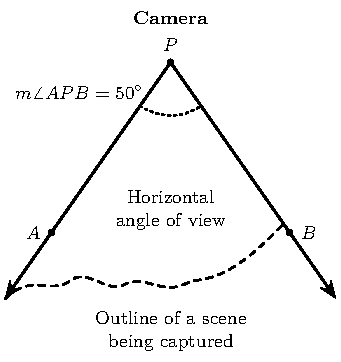
\includegraphics[width=.8\linewidth]{../figures/fhsm_2009_p56_f1.pdf}
    \end{center}

    Shelly wants to take an artistic photo of the decorated side of a building that sits on a flat plot of land. She wants to capture a level shot of the full width of the building (exactly), but she does not care whether the full building height is in the picture. So the horizontal expanse of the picture is fixed.\vspace{\baselineskip}

    She is using a camera lens with a fixed horizontal viewing angle of $50$ degrees, and she wants to take a level shot of the side of the building. She has found one spot that works, as indicated by point P in the figure at the right. Shelly believes that she could stand at other places to capture the same horizontal expanse but from a different perspective. Before she snaps the picture, she wants to examine some of those other positions. Your task is to figure out the ground locations where Shelly could stand to create a picture fitting her criteria.

    \begin{center}
      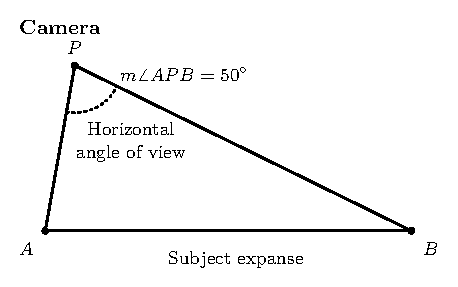
\includegraphics[width=.92\linewidth]{../figures/fhsm_2009_p57_f1.pdf}
    \end{center}

    Explore the situation, write down any conjectures you have regarding possible positions, and justify any that you can. The objective is to eventually create a conjecture describing the full range of possible positions. Prepare to clearly state your conjectures, as well as the thinking, exploration, and reasoning that explain how you arrived at them.

    \textbf{In the Classroom (Geometry Class)}

    An interactive drawing utility (with a file containing the sketch above), a hard copy of the sketch and a physical manipulative (a rigid angle---e.g., the expanse of a rigid compass), or a real camera and wall could be used to facilitate exploration of possible locations. The lesson begins with a full-class discussion of initial thoughts. After some time for individual thought or explanation, the following dialogue ensues.

    \begin{scriptlist}
      \item [Teacher:] Do you have any immediate conjectures to suggest?
      
      \item [Student 1:] I think there is a point right in the middle where you could stand.
      
      \item [Teacher:] What do you mean by ``middle''?
      
      \item [Student 1:] I mean I would stand at a point in the diagram that would be the same distance from points $A$ and $B$.
      
      \item [Student 2:] Oh, that means the point would be somewhere on the perpendicular bisector of the segment $AB$, which represents the building side. This is because we have already learned that the perpendicular bisector of the segment is the collection of points that are equidistant from points $A$ and $B$.
      
      \item [Teacher:] How would you find such a point? 
    \end{scriptlist}

    The students engage in some more work.

    \begin{scriptlist}
      \item [Student 1:] I'd put a point on the perpendicular bisector of segment $AB$ and then move it back and forth until the angle exactly fit the segment.
      
      \item [Teacher:] Good, that gives some detail regarding how one might locate a second point. [The teacher writes down a conjecture that there is a possible vertex location on the perpendicular bisector of segment $AB$. This conjecture will be addressed in a subsequent discussion---beyond the confines of this example.] Are there other ideas about possible vertices?
        
      \begin{center}
        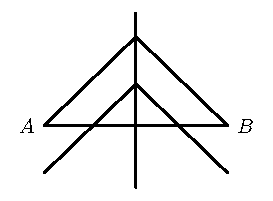
\includegraphics[width=.92\linewidth]{../figures/fhsm_2009_p57_2.pdf}
      \end{center}

      \item [Student 2:] Based on my experience with a camera, I think there would be many points where one could stand to show the entire building side.
    \end{scriptlist}

    Many students in the class agree with the conjecture that many points would work. Another student jumps in and suggests that that the possible positions possess symmetry. Eventually, someone states that reflective symmetry would be evident in the collection of possible points across the perpendicular bisector of $AB$. This conjecture will be evaluated subsequently, as well.

    \begin{scriptlist}
      \item [Teacher:] Now, by using either the interactive drawing utility or the physical manipulative, plot a collection of points that represent where the photographer might stand to snap the required image. See if any other conjectures emerge from this exploration.
      
      \item [Student 4:] [After some exploration] All the points seem to be on a circular arc that goes from point $A$ to point $B$---even though the photographer can't stand there.
    \end{scriptlist}

    The teacher next facilitates a discussion about stating in abstract terms what we refer to as the major conjecture: ``Given a line segment $AB$ and a specified side of line $AB$, each point, $P$, on the specified side of $AB$ with the property that $m\angle APB = 50^\circ$ lies on a circular arc containing $A$ and $B$.''

    \begin{center}
      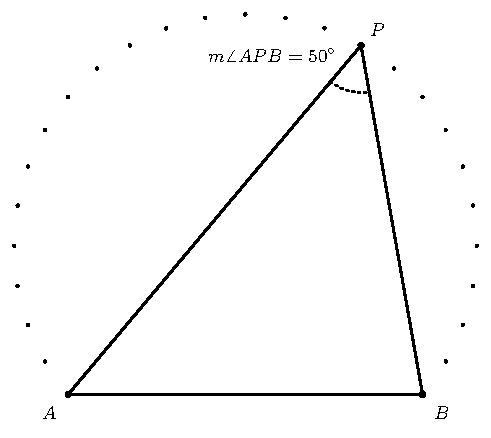
\includegraphics[width=.92\linewidth]{../figures/fhsm_2009_p58_1.pdf}
    \end{center}

    This conjecture is not resolved immediately. Rather, a set of questions is compiled by the class for moving toward a proof of this conjecture. These questions include the following:

    \begin{enumerate}
      \item Can we find out which circular arc we are talking about? That is, can we find the circle that contains this arc?
      
      \item Would every point on the arc (except points $A$ and $B$) represent possible positions where the photographer could stand?
      
      \item Would the arc miss any possible points?
    \end{enumerate}\vspace{\baselineskip}

    (See example 15 along with the supporting topic book on geometry for a full discussion of the conjecture.)

    \textbf{Key Elements of Mathematics}

    \begin{hanglist}
      \hangitem{Reasoning with Geometry---Conjecturing about geometric objects; Multiple geometric approaches}
    \end{hanglist}

    \textbf{Reasoning Habits}

    \begin{hanglist}
      \hangitem{Analyzing the problem---identifying relevant concepts, representations, or procedures; looking for hidden structure; considering special cases or simpler analogs; seeking patterns and relationships; making preliminary deductions and conjectures}

      \hangitem{Implementing a strategy-monitoring progress toward a solution; making logical deductions}
    \end{hanglist}
  }
  {
    Đứng đâu để chụp?
  }
  {
    \textbf{Task}

    Trong nhiếp ảnh, ``góc nhìn ngang'' mô tả độ mở góc của cảnh được thu vào ảnh, với đỉnh góc là ống kính máy ảnh. (Xem hình bên dưới, biểu diễn mặt phẳng ngang của cảnh chụp.) \vspace{\baselineskip}

    \begin{center}
      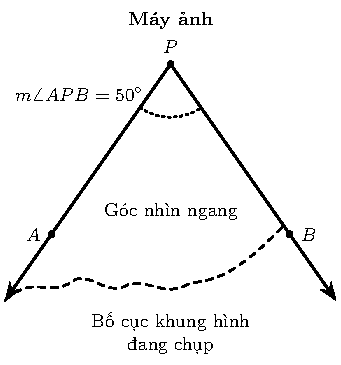
\includegraphics[width=.8\linewidth]{../figures/fhsm_2009_p56_f1_vi.pdf}
    \end{center}

    Shelly muốn chụp một bức ảnh nghệ thuật mặt bên được trang trí của tòa nhà nằm trên khu đất bằng phẳng. Cô muốn ghi lại trọn vẹn và chính xác bề rộng tòa nhà trong một bức ảnh ngang, nhưng không quan tâm liệu toàn bộ chiều cao tòa nhà có xuất hiện trong ảnh hay không. Do đó, khoảng mở ngang của ảnh được cố định. 

    Cô đang sử dụng ống kính có góc nhìn ngang cố định $50$ độ và muốn chụp ngang mặt bên tòa nhà. Cô đã tìm được một vị trí phù hợp, kí hiệu là điểm $P$ trong hình bên dưới. Shelly tin rằng cô có thể đứng ở vị trí khác để ghi lại cùng khoảng mở ngang ấy nhưng từ góc nhìn khác. Trước khi bấm máy, cô muốn xem xét một số vị trí khác như vậy. Nhiệm vụ của em là xác định các vị trí trên mặt đất mà Shelly có thể đứng để tạo ra bức ảnh thỏa mãn các tiêu chí đã nêu. \vspace{2\baselineskip}

    \begin{center}
      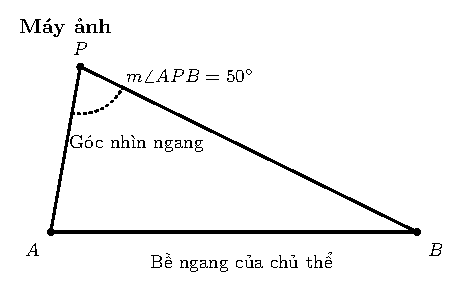
\includegraphics[width=.92\linewidth]{../figures/fhsm_2009_p57_f1_vi.pdf}
    \end{center}

    Hãy khám phá tình huống, ghi lại mọi phỏng đoán em có về các vị trí khả dĩ, và biện minh những phỏng đoán có thể biện minh được. Mục tiêu cuối cùng là hình thành phỏng đoán mô tả đầy đủ phạm vi các vị trí khả dĩ. Hãy chuẩn bị để trình bày rõ ràng phỏng đoán của em, cũng như quá trình suy nghĩ, khám phá và luận đã giúp em đi đến phỏng đoán ấy.

    \textbf{Trong lớp học (lớp hình học)}

    Công cụ vẽ tương tác (với tệp chứa hình phác thảo như trên), bản in của hình phác thảo và học cụ thao tác vật lí (một góc cứng---chẳng hạn, độ mở của compa được giữ cố định), hoặc máy ảnh thật và bức tường đều có thể được sử dụng để hỗ trợ việc khám phá vị trí khả dĩ. Bài học bắt đầu bằng cuộc thảo luận chung của cả lớp về những suy nghĩ ban đầu. Sau một khoảng thời gian để suy nghĩ hoặc giải thích cá nhân, cuộc đối thoại sau đây diễn ra.

    \begin{scriptlist}
      \item [Giáo viên:] Các em có phỏng đoán ban đầu nào muốn đề xuất không?

      \item [Học sinh 1:] Em nghĩ có một điểm ngay ở giữa mà ta có thể đứng.\vspace{\baselineskip}

      \item [Giáo viên:] Em muốn nói gì khi nói ``ở giữa''?

      \item [Học sinh 1:] Ý em là em sẽ đứng tại một điểm trong hình sao cho khoảng cách từ điểm đó đến $A$ và $B$ bằng nhau.

      \item [Học sinh 2:] À, vậy có nghĩa là điểm ấy sẽ nằm đâu đó trên đường trung trực của đoạn thẳng $AB$, đoạn thẳng biểu diễn mặt bên của tòa nhà. Điều này là vì ta đã học rằng đường trung trực của một đoạn thẳng là tập hợp các điểm cách đều hai đầu mút của đoạn thẳng đó, tức là cách đều hai điểm $A$ và $B$.
      
      \item [Giáo viên:] Em sẽ tìm một điểm như vậy bằng cách nào? 
    \end{scriptlist}

    Học sinh tiếp tục làm việc thêm một lúc.

    \begin{scriptlist}
      \item [Học sinh 1:] Em sẽ đặt một điểm trên đường trung trực của đoạn $AB$ rồi di chuyển nó tới lui cho đến khi góc vừa khít với đoạn thẳng.
      
      \item [Giáo viên:] Tốt, điều đó cho ta thêm một số chi tiết về cách có thể xác định một điểm thứ hai. [Giáo viên ghi lại phỏng đoán rằng có một vị trí đỉnh khả dĩ trên đường trung trực của đoạn $AB$. Phỏng đoán này sẽ được bàn đến trong một thảo luận về sau, nằm ngoài phạm vi của ví dụ này.] Còn ý tưởng nào khác về các đỉnh khả dĩ không?\vspace{2\baselineskip}
        
      \begin{center}
        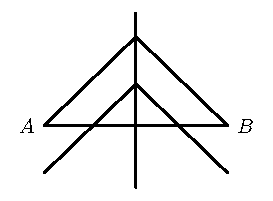
\includegraphics[width=.92\linewidth]{../figures/fhsm_2009_p57_2.pdf}
      \end{center}

      \item [Học sinh 2:] Dựa trên kinh nghiệm của em với máy ảnh, em nghĩ sẽ có nhiều điểm mà người ta có thể đứng để chụp trọn mặt bên của tòa nhà.
    \end{scriptlist}

    Nhiều học sinh trong lớp đồng ý với phỏng đoán rằng nhiều điểm có thể phù hợp. Một học sinh khác tham gia và gợi ý rằng các vị trí khả dĩ có tính đối xứng. Cuối cùng, có người phát biểu rằng tập hợp các điểm khả dĩ sẽ có đối xứng gương qua đường trung trực của $AB$. Phỏng đoán này cũng sẽ được thẩm định sau đó.\vspace{\baselineskip}

    \begin{scriptlist}
      \item [Giáo viên:] Bây giờ, bằng cách sử dụng công cụ vẽ tương tác hoặc học cụ thao tác vật lí, hãy đánh dấu một tập hợp điểm biểu diễn vị trí mà nhiếp ảnh gia có thể đứng để chụp bức ảnh theo yêu cầu. Hãy xem liệu có phỏng đoán nào khác xuất hiện từ quá trình khám phá này không.
      
      \item [Học sinh 4:] [Sau một thời gian khám phá] Tất cả các điểm dường như đều nằm trên một cung tròn đi từ điểm $A$ đến điểm $B$---mặc dù nhiếp ảnh gia không thể đứng tại đó.  
    \end{scriptlist}

    Sau đó, giáo viên điều phối cuộc thảo luận về việc phát biểu bằng ngôn ngữ trừu tượng cái mà ta gọi là phỏng đoán chính: ``Cho đoạn thẳng $AB$ và một phía xác định của đường thẳng $AB$, mỗi điểm $P$ nằm về phía đã xác định của $AB$ và thỏa mãn điều kiện $m\angle APB = 50^\circ$ đều nằm trên một cung tròn chứa $A$ và $B$.''

    \begin{center}
        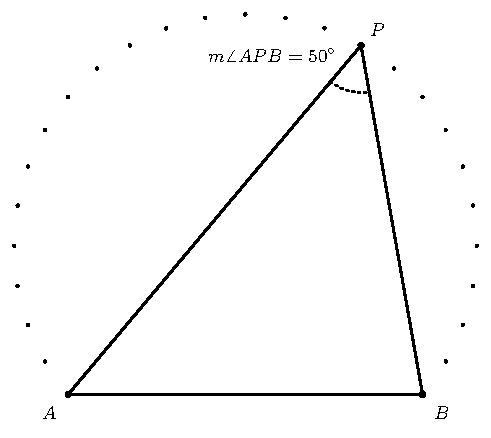
\includegraphics[width=.92\linewidth]{../figures/fhsm_2009_p58_1.pdf}
    \end{center}

    Phỏng đoán này không được giải quyết ngay lập tức. Thay vào đó, lớp học tập hợp một bộ câu hỏi để tiến tới chứng minh phỏng đoán này. Các câu hỏi đó bao gồm:

    \begin{enumerate}
      \item Ta có thể xác định cung tròn đang nói đến là cung nào không? Tức là, ta có thể tìm được đường tròn chứa cung đó không?
      
      \item Liệu mọi điểm trên cung, trừ các điểm $A$ và $B$, có biểu diễn vị trí khả dĩ nơi nhiếp ảnh gia có thể đứng không?
      
      \item Liệu cung ấy có bỏ sót vị trí khả dĩ nào không?
    \end{enumerate}

    (Xem Ví dụ 15 cùng với sách chủ đề bổ trợ về hình học để có thảo luận đầy đủ về phỏng đoán này.)

    \textbf{Các yếu tố then chốt của toán học}

    \begin{hanglist}
      \hangitem{Luận với hình học---Phỏng đoán về các đối tượng hình học; Nhiều cách tiếp cận hình học}
    \end{hanglist}

    \textbf{Thói quen luận}

    \begin{hanglist}
      \hangitem{Phân tích bài toán---xác định khái niệm, thủ tục hoặc biểu diễn toán học thích đáng; tìm kiếm cấu trúc ẩn; xét trường hợp đặc biệt hoặc dạng tương tự đơn giản hơn; tìm kiếm mẫu hình và quan hệ; đưa ra suy diễn và phỏng đoán sơ bộ}

      \hangitem{Triển khai chiến lược---theo dõi tiến trình đi đến lời giải; thực hiện suy diễn logic}
    \end{hanglist}
  }{}

\ParallelSection
  {Construction and Evaluation of Geometric Arguments}
  {Xây dựng và thẩm định các lập luận hình học}
  {}

\TriPara
  {
    \EN{Making a conjecture, as in example 14, is a first step in mathematical inquiry. Students need to follow up many of their conjectures with efforts to either justify or disprove them. Although the major conjecture in example 14 is not resolved immediately, the activity leads naturally to the development of several important geometric results that emerge from question 1 in the example. In particular, the students in example 15 make progress toward resolving the conjecture by establishing the fact that three noncollinear points in the plane lie on a unique circle. Further progress is made when students prove the inscribed angle theorem, which states that every point, $P$, on the conjectured circular arc would satisfy the condition that $m\angle APB$ equals $50$ degrees. However, students would still need to prove that no other point on the same side of line AB could be the vertex of such an angle. Example 15 also exemplifies the reasoning habit of looking for hidden structure---in this example, an auxiliary line.}
  }
  {
    \VI{Việc đưa ra phỏng đoán, như trong Ví dụ 14, là bước khởi đầu của hoạt động tìm tòi toán học. Học sinh cần tiếp tục theo đuổi nhiều phỏng đoán của mình bằng nỗ lực biện minh hoặc bác bỏ các phỏng đoán ấy. Mặc dù phỏng đoán chính trong Ví dụ 14 không được giải quyết ngay lập tức, hoạt động này dẫn tự nhiên tới việc phát triển một số kết quả hình học quan trọng nảy sinh từ câu hỏi thứ nhất trong ví dụ. Cụ thể, trong Ví dụ 15, học sinh tiến thêm một bước trong việc giải quyết phỏng đoán bằng cách xác lập kết quả rằng ba điểm không thẳng hàng trong mặt phẳng nằm trên đúng một đường tròn. Tiến triển tiếp theo đạt được khi học sinh chứng minh định lí góc nội tiếp, theo đó mọi điểm $P$ nằm trên cung tròn được phỏng đoán đều thỏa mãn điều kiện $m\angle APB$ bằng $50^\circ$. Tuy nhiên, học sinh vẫn cần chứng minh rằng không có điểm nào khác nằm về cùng một phía của đường thẳng $AB$ có thể là đỉnh của một góc như vậy. Ví dụ 15 cũng minh họa thói quen luận tìm kiếm cấu trúc ẩn---trong trường hợp này là một đường phụ trợ.}
  }{\NOTE{}}

\TriPara
  {
    \EN{The progress in levels of reasoning can clearly be seen in these two examples. Students begin with explorations at the empirical level, moving to the preformal level as students suggest initial conclusions that can be drawn, such as that the arc actually passes through endpoints $A$ and $B$. Example 15 picks up the discussion with increasingly formal reasoning, culminating in conclusions supported by formal proof.}
  }
  {
    \VI{Sự phát triển qua các mức luận được thể hiện rõ trong hai ví dụ này. Học sinh khởi đầu bằng hoạt động khám phá ở mức thực nghiệm, rồi chuyển sang mức tiền hình thức khi các em đề xuất những kết luận ban đầu có thể rút ra, chẳng hạn như cung ấy thật sự đi qua hai đầu mút $A$ và $B$. Ví dụ 15 tiếp nối cuộc thảo luận bằng luận ngày càng mang tính hình thức, đỉnh điểm là những kết luận được hỗ trợ bằng chứng minh hình thức.}
  }{\NOTE{}}


\TriExample
  {
    Circle of Points
  }
  {
    \textbf{Task}

    This task answers question 1 raised at the end of example 14, ``Picture This'': What circle contains the conjectured arc?

    \begin{center}
      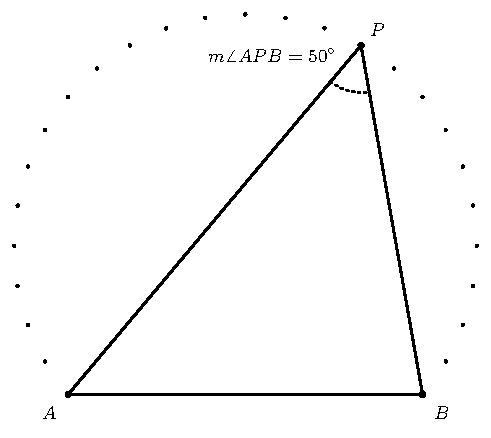
\includegraphics[width=.92\linewidth]{../figures/fhsm_2009_p58_1.pdf}
    \end{center}

    \textbf{In the Classroom (Geometry Class)}

    Students are divided into groups with the assignment to decide what to do next. After a short time, the groups report on possible strategies:

    \begin{scriptlist}
      \item [Group 1:] We think you need to find the center and radius of the circle.
      
      \item [Group 2:] We think you just need to find the center of the circle. You don't need to find the radius, because you already know at least one point on the circle---either the point $P$ specified in the original problem or points $A$ or $B$, which are part of the conjecture. You can use the center and one of these points on the circle to draw the whole circle.
      
      \item [Group 3:] We think you need the center. We think the center should be a point on segment $AB$ halfway between $A$ and $B$. The radius should be half the length of segment $AB$.
    \end{scriptlist}

    The groups reconvene to discuss these and possibly other thoughts. After a few more minutes the groups report.

    \begin{scriptlist}
      \item [Group 4:] We tested to see if the midpoint of segment $AB$ would be the center. The circle did not go through the point $P$ we were given, so the midpoint is not the center in this case. So next we used the interactive drawing utility to try to create the circle that fit the points and figure out its center. We got a pretty good circle. We didn't think it would fit all the points because we just approximated the locations of points that would be vertices of 50 degree angles when we made them. But we are even more convinced that there is a circle through the point $P$, which we were using for the 50 degree angle, and points $A$ and $B$---and all actual real points where the photographer could stand.
      
        \begin{center}
          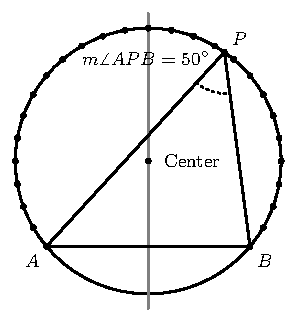
\includegraphics[width=.92\linewidth]{../figures/fhsm_2009_p60_f1.pdf}
        \end{center}

      We then tried to think about the center and agreed that the center (like the midpoint of segment $AB$) needs to be equidistant from both $A$ and $B$, since the circle goes through $A$ and $B$. Thinking back to what we talked about when we started example 14, we conclude that the center of the circle has to be on the perpendicular bisector of segment $AB$. We added the perpendicular bisector of segment $AB$ to our drawing, and it went right through the center of the circle we had drawn---just like it was supposed to!

      Then someone else in our group noticed that the same reasoning works with the two points $A$ and $P$. That is, since the circle goes through $A$ and $P$, its center would have to lie on the perpendicular bisector of the segment $AP$, as well. We added the perpendicular bisector of segment $AP$ to our sketch, constructed these two bisectors, and found that they intersect in one point, which we called $G$. That is the only point that lies on both perpendicular bisectors.

      So it is the only possible point for the center of a circle. So we could now draw the circle by choosing the center and any one of the points $A$, $P$, or $B$.\vspace{\baselineskip}

      \item [Teacher:] Before you draw your circle, let me ask you a question. It seems that you have shown that if there is a circle through the points $P$, $A$, and $B$, the center must be $G$. Can you or any other group prove that there will definitely be such a circle---that you weren't just lucky this time with these particular points or that the drawing is misleading? Let's work on that in our groups.  
    \end{scriptlist}\vspace{2\baselineskip}

    After a few minutes, a new group is ready to contribute its proof:

    \begin{scriptlist}
      \item [Group 5:] We are assuming that we have the three noncollinear points $P$, $A$, and $B$ and that $G$ is the point of intersection of the perpendicular bisectors of sides $AB$ and $AP$-like we have been talking about. We will show that $G$ is the center of a circle that goes through points $P$, $A$, and $B$. Construct segments $GP$, $GA$, and $GB$. Segments $GP$ and $GA$ have to have equal lengths because $G$ is on the perpendicular bisector of segment $AP$. Segments $GA$ and $GB$ must be equal in length because $G$ is on the perpendicular bisector of segment $AB$. Since both segments $GP$ and $GB$ are equal in length to segment $GA$, all three segments have equal length. So if we draw the circle with center $G$ and radius equal to the length of segment $GA$, the circle will definitely go through the three points $A$, $B$, and $P$.

      \begin{center}
        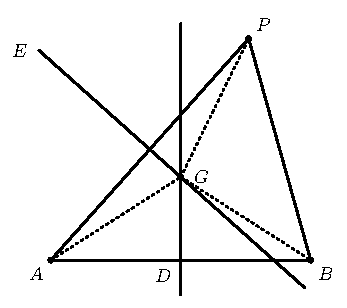
\includegraphics[width=.92\linewidth]{../figures/fhsm_2009_p61_1.pdf}
      \end{center}
    \end{scriptlist}

    The teacher asks for comments and critiques from the class with regard to group 5's presentation. (There are none.) The teacher then proposes that the day's discussion suggests three results: (1) Three noncollinear points in the plane determine a unique circle. (2) (Circle construction algorithm) The center of that circle can be found by finding the point of intersection of the perpendicular bisectors of any two sides of the triangle that has the three noncollinear points as vertices. (3) The perpendicular bisectors of the three sides of a triangle intersect in a single point. The first two of these results comes directly from the discussion. The third is closely related.

    For homework, students are asked to write proofs of the first and third statements. In some instances this assignment requires organization, generalization, or extension of arguments given in the discussion. In others it involves adding detail. For the second statement, the students are asked to write an algorithm (i.e., well-defined sequence of steps) for constructing a circle through three noncollinear points in the plane.\vspace{\baselineskip}

    \textbf{Key Elements}

    \begin{hanglist}
      \hangitem{Reasoning with Geometry---Construction and evaluation of geometric arguments}
    \end{hanglist}

    \textbf{Reasoning Habits}

    \begin{hanglist}
      \hangitem{Analyzing a problem---identifying relevant mathematical concepts, representations, or procedures; looking for hidden structure}

      \hangitem{Implementing a strategy ---- organizing a solution; making logical deductions; monitoring progress toward a solution}

      \hangitem{Reflecting on a solution ---- justifying or validating a solution}
    \end{hanglist}
  }
  {
    Tâm ở đâu?
  }
  {
    \textbf{Nhiệm vụ}

    Nhiệm vụ này trả lời câu hỏi 1 được nêu ở cuối Ví dụ 14, ``Đứng đâu để chụp?'': Đường tròn nào chứa cung được phỏng đoán?

    \begin{center}
      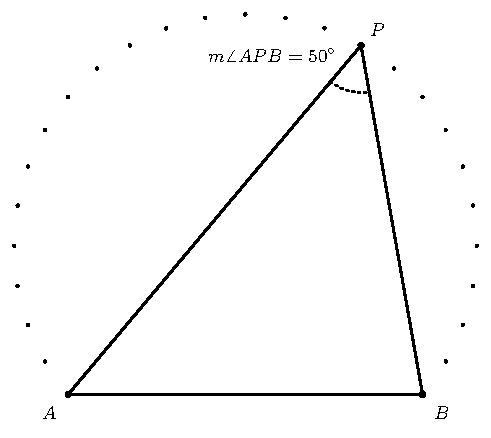
\includegraphics[width=.92\linewidth]{../figures/fhsm_2009_p58_1.pdf}
    \end{center}

    \textbf{Trong lớp học (lớp hình học)}

    Học sinh được chia thành nhóm và được giao nhiệm vụ quyết định bước tiếp theo cần thực hiện. Sau một thời gian ngắn, các nhóm báo cáo về những chiến lược khả dĩ:

    \begin{scriptlist}
      \item [Nhóm 1:] Chúng em nghĩ cần tìm tâm và bán kính của đường tròn.
      
      \item [Nhóm 2:] Chúng em nghĩ chỉ cần tìm tâm của đường tròn. Không cần tìm bán kính, vì đã biết ít nhất một điểm nằm trên đường tròn---hoặc điểm $P$ được cho trong bài toán ban đầu, hoặc điểm $A$ hay $B$, vốn là một phần của phỏng đoán. Ta có thể dùng tâm và một trong những điểm này trên đường tròn để vẽ toàn bộ đường tròn.\vspace{\baselineskip}
      
      \item [Nhóm 3:] Chúng em nghĩ cần tìm tâm. Chúng em nghĩ tâm phải là điểm nằm trên đoạn $AB$, ở chính giữa $A$ và $B$. Bán kính sẽ bằng một nửa độ dài đoạn $AB$. 
    \end{scriptlist}

    Các nhóm họp lại để thảo luận về những ý tưởng này và những suy nghĩ khác có thể có. Sau vài phút nữa, các nhóm báo cáo tiếp.

    \begin{scriptlist}
      \item [Nhóm 4:] Chúng em kiểm tra xem trung điểm của đoạn $AB$ có phải là tâm không. Đường tròn không đi qua điểm $P$ đã cho, nên trong trường hợp này trung điểm không phải là tâm. Vì vậy, tiếp theo chúng em dùng công cụ vẽ tương tác để thử dựng đường tròn đi qua các điểm đã cho và tìm tâm của nó. Chúng em dựng được một đường tròn khá sát. Chúng em không nghĩ nó sẽ đi qua chính xác mọi điểm, vì khi tạo các điểm ấy, chúng em chỉ ước lượng vị trí của những điểm có thể là đỉnh của góc $50$ độ. Nhưng chúng em càng tin chắc hơn rằng có một đường tròn đi qua điểm $P$, điểm mà chúng em dùng cho góc $50$ độ, và các điểm $A$ và $B$---cũng như mọi vị trí thật sự mà nhiếp ảnh gia có thể đứng.\vspace{\baselineskip}
      
      \begin{center}
        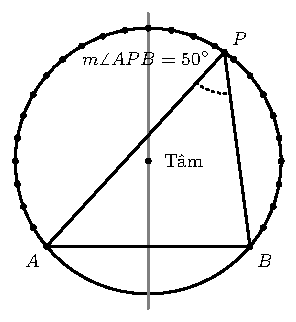
\includegraphics[width=.92\linewidth]{../figures/fhsm_2009_p60_f1_vi.pdf}
      \end{center}

      Sau đó, chúng em suy nghĩ về tâm và thống nhất rằng tâm (cũng như trung điểm của đoạn $AB$) cần cách đều cả $A$ và $B$, vì đường tròn đi qua $A$ và $B$. Nhớ lại điều đã bàn khi bắt đầu Ví dụ 14, chúng em kết luận rằng tâm của đường tròn phải nằm trên đường trung trực của đoạn $AB$. Chúng em thêm đường trung trực của đoạn $AB$ vào hình vẽ, và nó đi đúng qua tâm của đường tròn mà chúng em đã dựng---đúng như dự kiến!\vspace{3\baselineskip}

      Rồi một bạn khác trong nhóm nhận ra rằng cách luận ấy cũng đúng với hai điểm $A$ và $P$. Nghĩa là, vì đường tròn đi qua $A$ và $P$, nên tâm của nó cũng phải nằm trên đường trung trực của đoạn $AP$. Chúng em thêm đường trung trực của đoạn $AP$ vào phác thảo, dựng hai đường trung trực ấy, và thấy chúng cắt nhau tại một điểm, chúng em gọi là $G$. Đó là điểm duy nhất nằm trên cả hai đường trung trực.\vspace{2\baselineskip}

      Vì thế, đó là điểm duy nhất có thể là tâm của đường tròn. Do đó, bây giờ chúng em có thể vẽ đường tròn bằng cách chọn tâm và bất kì điểm nào trong các điểm $A$, $P$, hoặc $B$.

      \item [Giáo viên:] Trước khi các em vẽ đường tròn, thầy hỏi một câu. Có vẻ như các em đã chỉ ra rằng nếu có một đường tròn đi qua các điểm $P$, $A$, và $B$, thì tâm của nó phải là $G$. Các em hoặc nhóm nào khác có thể chứng minh rằng chắc chắn sẽ có một đường tròn như vậy không---rằng lần này các em không chỉ tình cờ gặp may với những điểm cụ thể này, và hình vẽ cũng không đánh lừa ta? Hãy tiếp tục làm việc trong nhóm về điều đó.
    \end{scriptlist}

    Sau vài phút, một nhóm mới đã sẵn sàng đóng góp chứng minh:

    \begin{scriptlist}
      \item [Nhóm 5:] Chúng em giả sử rằng ta có ba điểm không thẳng hàng $P$, $A$ và $B$, và $G$ là giao điểm của các đường trung trực của hai cạnh $AB$ và $AP$, giống như điều chúng ta vừa trao đổi. Chúng em sẽ chỉ ra rằng $G$ là tâm của một đường tròn đi qua ba điểm $P$, $A$ và $B$. Dựng các đoạn thẳng $GP$, $GA$ và $GB$. Hai đoạn thẳng $GP$ và $GA$ phải có cùng độ dài vì $G$ nằm trên đường trung trực của đoạn $AP$. Hai đoạn thẳng $GA$ và $GB$ cũng phải có cùng độ dài vì $G$ nằm trên đường trung trực của đoạn $AB$. Vì cả hai đoạn thẳng $GP$ và $GB$ đều có cùng độ dài với đoạn $GA$, nên cả ba đoạn thẳng có cùng độ dài. Do đó, nếu ta vẽ đường tròn tâm $G$ với bán kính bằng độ dài đoạn $GA$, thì đường tròn ấy chắc chắn sẽ đi qua ba điểm $A$, $B$ và $P$.
      
      \begin{center}
        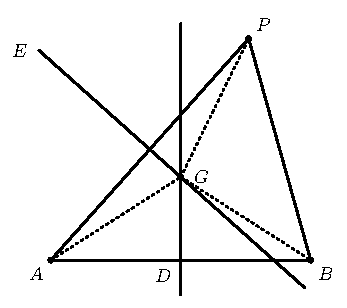
\includegraphics[width=.92\linewidth]{../figures/fhsm_2009_p61_1.pdf}
      \end{center}
    \end{scriptlist}

    Giáo viên yêu cầu cả lớp nhận xét và phản biện phần trình bày của Nhóm 5. (Không có ý kiến nào.) Sau đó, giáo viên đề xuất rằng cuộc thảo luận trong ngày gợi ra ba kết quả: (1) Ba điểm không thẳng hàng trong mặt phẳng xác định một đường tròn duy nhất. (2) (Thuật toán dựng đường tròn) Tâm của đường tròn ấy có thể được tìm bằng cách xác định giao điểm của các đường trung trực của bất kì hai cạnh nào trong tam giác có ba điểm không thẳng hàng ấy làm đỉnh. (3) Các đường trung trực của ba cạnh của một tam giác cắt nhau tại một điểm. Hai kết quả đầu tiên rút ra trực tiếp từ cuộc thảo luận. Kết quả thứ ba có liên hệ gần.

    Về nhà, học sinh được yêu cầu viết chứng minh cho mệnh đề thứ nhất và thứ ba. Trong một số trường hợp, nhiệm vụ này đòi hỏi phải tổ chức lại, khái quát hóa, hoặc mở rộng các lập luận đã nêu trong cuộc thảo luận. Trong trường hợp khác, nhiệm vụ đòi hỏi bổ sung chi tiết. Với mệnh đề thứ hai, học sinh được yêu cầu viết một thuật toán, tức là một dãy bước được xác định rõ ràng, để dựng đường tròn đi qua ba điểm không thẳng hàng trong mặt phẳng.

    \textbf{Các yếu tố then chốt của toán học}

    \begin{hanglist}
      \hangitem{Luận với hình học---Xây dựng và thẩm định các lập luận hình học}
    \end{hanglist}

    \textbf{Thói quen luận}

    \begin{hanglist}
      \hangitem{Phân tích bài toán---xác định khái niệm, thủ tục hoặc biểu diễn toán học thích đáng; tìm kiếm cấu trúc ẩn}\vspace{\baselineskip}

      \hangitem{Triển khai chiến lược---tổ chức lời giải; thực hiện suy diễn logic; theo dõi tiến trình đi đến lời giải}

      \hangitem{Phản tư về lời giải---biện minh hoặc kiểm chứng lời giải}
    \end{hanglist}
  }{}


\TriPara
  {
    \EN{The validity of a proof is not determined by how it is presented. A two-column proof is not necessarily more valid (or rigorous) than a proof given in paragraph form. In fact, strict adherence to a specific proof format may elevate focus on form over function, thus obstructing the creative mix of reasoning habits and ultimately hindering the chance of students' successfully understanding the mathematical consequences of the arguments (Herbst 2002). In addition to facility in constructing chains of reasoning, constructing a mathematical proof often requires resourcefulness in selecting a strategy, cultured intuition, and good judgment. Blind alleys and false starts sometimes generate insight along with the inevitable frustration that accompanies them---therein lies the challenge!}
  }
  {
    \VI{Tính hiệu lực của chứng minh không được quyết định bởi cách trình bày. Chứng minh hai cột không nhất thiết hiệu lực hơn, hay chặt chẽ hơn, so với chứng minh được viết dưới dạng đoạn văn. Thực ra, việc tuân thủ cứng nhắc một khuôn mẫu trình bày chứng minh cụ thể có thể đặt hình thức lên trên chức năng, qua đó cản trở sự kết hợp sáng tạo giữa các thói quen luận và rốt cuộc làm giảm cơ hội để học sinh hiểu thành công các hệ quả toán học của những lập luận ấy (Herbst 2002). Ngoài khả năng xây dựng chuỗi luận, việc xây dựng chứng minh toán học còn thường đòi hỏi sự linh hoạt trong lựa chọn chiến lược, trực giác được nuôi dưỡng, và khả năng phán đoán tốt. Những ngõ cụt và khởi đầu sai hướng đôi khi vẫn đem lại soi sáng, cùng với nỗi bực bội tất yếu đi kèm---chính đó là thách thức!}
  }{\NOTE{}}

\ParallelSection
  {Multiple Geometric Approaches}
  {Nhiều cách tiếp cận hình học}
  {}

\TriPara
  {
    \EN{Geometric situations can be approached in many different ways, including the synthetic approach seen in examples 14 and 15 and the coordinate approach seen in the example involving the distance formula in chapter 1. The coordinate approach applies algebraic concepts in geometric contexts, and vice versa.}
  }
  {
    \VI{Các tình huống hình học có thể được tiếp cận theo nhiều cách khác nhau, bao gồm cách tiếp cận tổng hợp được thể hiện trong Ví dụ 14 và 15, cũng như cách tiếp cận tọa độ được minh họa trong ví dụ liên quan đến công thức khoảng cách ở Chương 1. Cách tiếp cận tọa độ vận dụng khái niệm đại số trong ngữ cảnh hình học, đồng thời vận dụng khái niệm hình học trong ngữ cảnh đại số.}
  }{\NOTE{}}

\TriPara
  {
    \EN{The value of transformations in geometry has been recognized for more than thirty years (cf. Coxford and Usiskin [1971]; NCTM [1989, 2000a]), although they continue to receive limited attention in many curricula. Geometric transformations---rotations, translations, reflections, and dilations---provide another useful approach to understanding geometric relationships. The transformation approach to geometry supports an alternative way of considering congruence, similarity, and symmetry. In example 16, students are challenged to go beyond simple but misleading rules and think carefully about rotational symmetry. Example 16 also exemplifies the reasoning habit of monitoring one's progress, including considering approaches taken by other members of the class.}
  }
  {
    \VI{Giá trị của các phép biến hình trong hình học đã được thừa nhận trong hơn ba thập niên qua (xem Coxford and Usiskin [1971]; NCTM [1989, 2000a]), mặc dù trong nhiều chương trình học, chúng vẫn chưa được chú ý tương xứng. Các phép biến hình hình học---bao gồm phép quay, phép tịnh tiến, phép đối xứng và phép vị tự---cung cấp thêm một cách tiếp cận hữu ích để hiểu các quan hệ hình học. Cách tiếp cận hình học bằng phép biến hình hỗ trợ một cách khác để xem xét tính bằng nhau, đồng dạng và đối xứng. Trong Ví dụ 16, học sinh được thử thách vượt qua những quy tắc đơn giản nhưng dễ gây hiểu lầm, để suy nghĩ cẩn trọng về đối xứng quay. Ví dụ 16 cũng minh họa thói quen luận theo dõi tiến trình của bản thân, kể cả khi xem xét cách làm của các bạn trong lớp.}
  }
  {
    \NOTE{Phép biến hình từ lâu đã được xem là có giá trị trong dạy học hình học, nhưng trong thực tế chương trình học, chúng vẫn chưa được dành vị trí tương xứng. Vì thế, điều cần thấy ở đây là khoảng cách giữa điều đã được thừa nhận về mặt định hướng và điều thật sự được triển khai trong lớp học.

    Điểm khác biệt của cách tiếp cận này nằm ở chỗ nó cho học sinh hiểu các quan hệ hình học qua sự biến đổi của hình. Khi nhìn hình qua phép quay, phép tịnh tiến, phép đối xứng hay phép vị tự, học sinh không chỉ xét hình ``là gì'', mà còn xét hình ``biến thành gì'' và ``điều gì vẫn được giữ lại''. Nhờ đó, những khái niệm như bằng nhau, đồng dạng và đối xứng không chỉ được nhận biết bằng dấu hiệu tĩnh, mà còn được hiểu qua quan hệ bảo toàn.

    Đối xứng quay là trường hợp dễ làm lộ sự khác biệt giữa học thuộc quy tắc và hiểu bản chất. Những quy tắc ngắn gọn thường có thể giúp nhận dạng nhanh, nhưng cũng dễ dẫn tới kết luận sai nếu không kiểm tra kĩ điều kiện của tình huống. Vì vậy, việc buộc học sinh suy nghĩ cẩn thận hơn về đối xứng quay không chỉ nhằm sửa nhầm lẫn cục bộ, mà còn nhằm rèn luyện cách học hình học có kiểm soát hơn.

    Việc theo dõi tiến trình của bản thân cũng hiện rõ ở đây. Khi cách làm chưa đủ vững, học sinh cần biết dừng lại, xem lại, và đối chiếu với cách làm khác trong lớp. Chính sự điều chỉnh ấy giúp quá trình tìm hiểu hình học không dừng ở phản ứng theo thói quen, mà tiến dần tới chỗ hiểu chắc hơn vì sao kết luận là đúng.}
  }

\TriExample
  {
    Taking a Spin
  }
  {
    \textbf{Task}

    What regular polygons have 80-degree rotational symmetry?

    \textbf{In the Classroom (Geometry Class)}

    Students have been asked to answer the following problem for homework: ``What regular polygons have 80-degree rotational symmetry?'' (Martin 1996). At the beginning of class the following day, class members discuss this problem in small groups. One group goes to the front of the class to present its solution.

    \begin{scriptlist}
      \item [Student 1:] We concluded that there aren't any, since $80$ does not divide into $360$ evenly. When we were looking at regular polygons last week, we saw that if you have, like, a pentagon, you can make five triangles, and each has a 72-degree angle. So if you turn the triangle $72$ degrees, it will match. But you can't do that with $80$. So it won't work.\vspace{2\baselineskip}
      
      \item [Teacher:] What did the rest of the groups conclude?
      
      \item [Student 2:] That's what we thought at first. But then we thought about a 360-gon has a 1-degree angle and so it should be able to hit every degree, so if you rotate it $80$ times, it will eventually work!
      
      \item [Student 1:] But is that possible? Eighty doesn't divide into $360$, right?
    \end{scriptlist}\vspace{\baselineskip}

    The teacher asks the students to discuss this issue further in their small groups for a few minutes and then pulls the class back together, asking the groups to share their observations.

    \begin{scriptlist}
      \item [Student 3:] OK, we agree that $360$ will work. Like they said, it will hit every degree. [He draws a rough sketch with many small sides.] If you rotate it once, it will match. But you can keep on going. [He mimics doing lots of very small rotations.] And when you do this $80$ times, it will work.\vspace{2\baselineskip}
      
      \item [Teacher:] Is that really 80-degree rotational symmetry?
      
      \item [Student 3:] We rotated $80$ degrees, and it matched up with itself.
      
      \item [Student 4:] We think that $2$ degrees should work, too.
      
      \item [Teacher:] What do you think they mean by that?
      
      \item [Student 4:] If you rotate it forty times, it will hit $80$ degrees.
      
      \item [Student 5:] But you can't have a 2-gon! That wouldn't even be a polygon.
      
      \item [Student 4:] Oh.
      
      \item [Student 6:] It's not a $2$-gon, it has a 2 degree angle. So if you divide $2$ into $360$, that would be a 180-gon. 
    \end{scriptlist}

    The class continues to discuss the situation and finally agrees that both regular 360-gons and 180-gons will work. Students suggest other regular polygons that they think will work, and the teacher ends the discussion by assigning students the task of finding all regular polygons that have 80-degree rotational symmetry. He asks them to write up their findings in a short essay that they can share with their classmates the next day. The essay should both give all the regular polygons that they have found and prove that they have in fact found them all.

    \textbf{Key Elements of Mathematics}

    \begin{hanglist}
      \hangitem{Reasoning with Geometry---Conjecturing about geometric objects; Construction and evaluation of geometric arguments; Multiple geometric approaches}
    \end{hanglist}

    \textbf{Reasoning Habits}

    \begin{hanglist}
      \hangitem{Analyzing a problem---identifying concepts, representations, or procedures; considering special cases or simpler analogs}\vspace{\baselineskip}

      \hangitem{Implementing a strategy---monitoring progress toward a solution}

      \hangitem{Reflection on a solution---reconciling different approaches; justifying or validating a solution; refining arguments}
    \end{hanglist}
  }
  {
    Xoay đi!
  }
  {
    \textbf{Nhiệm vụ}

    Những đa giác đều nào có đối xứng quay góc 80 độ?

    \textbf{Trong lớp học (lớp hình học)}

    Học sinh được yêu cầu trả lời bài toán sau đây làm bài tập về nhà: ``Những đa giác đều nào có đối xứng quay 80 độ?'' (Martin 1996). Vào đầu giờ học ngày hôm sau, các thành viên trong lớp thảo luận bài toán này theo các nhóm nhỏ. Một nhóm lên trước lớp trình bày lời giải của mình.

    \begin{scriptlist}
      \item [Học sinh 1:] Chúng em kết luận rằng không có đa giác đều nào như vậy, vì $360$ không chia hết cho $80$. Khi tìm hiểu về đa giác đều tuần trước, chúng em thấy rằng, chẳng hạn với ngũ giác đều, ta có thể chia nó thành năm tam giác, và mỗi tam giác có một góc $72$ độ ở tâm. Vì vậy, nếu quay tam giác đi $72$ độ, nó sẽ khớp với vị trí kế tiếp. Nhưng ta không thể làm điều đó với $80$ độ. Vì vậy trường hợp này không được.

      \item [Giáo viên:] Các nhóm còn lại kết luận thế nào?
      
      \item [Học sinh 2:] Ban đầu chúng em cũng nghĩ vậy. Nhưng rồi chúng em nghĩ đến đa giác đều 360 cạnh: nó có góc quay 1 độ, nên có thể trùng khớp ở từng độ; vì vậy nếu quay nó $80$ lần thì cuối cùng cũng sẽ trùng khớp!
      
      \item [Học sinh 1:] Nhưng như vậy có được không? $360$ đâu có chia hết cho $80$, đúng không?
    \end{scriptlist}

    Giáo viên yêu cầu học sinh tiếp tục thảo luận vấn đề này trong nhóm nhỏ thêm vài phút, rồi tập hợp cả lớp lại và yêu cầu các nhóm chia sẻ quan sát của mình.\vspace{\baselineskip}

    \begin{scriptlist}
      \item [Học sinh 3:] Được rồi, chúng em đồng ý rằng đa giác đều 360 cạnh thỏa mãn. Như các bạn nói, nó sẽ khớp sau mỗi độ. [Bạn ấy vẽ một hình phác thảo thô với rất nhiều cạnh nhỏ.] Nếu quay một lần, nó sẽ khớp. Nhưng ta có thể tiếp tục quay. [Bạn ấy làm động tác quay rất nhiều lần với những góc rất nhỏ.] Và khi làm như vậy $80$ lần thì nó sẽ khớp.

      \item [Giáo viên:] Như vậy có thật sự là đối xứng quay góc 80 không không?

      \item [Học sinh 3:] Chúng em đã quay $80$ độ, và nó trùng khớp với chính nó.

      \item [Học sinh 4:] Chúng em nghĩ góc quay $2$ độ cũng được.

      \item [Giáo viên:] Em nghĩ các bạn ấy muốn nói gì khi nói như vậy?

      \item [Học sinh 4:] Nếu quay bốn mươi lần thì sẽ đạt đến $80$ độ.

      \item [Học sinh 5:] Nhưng không thể có đa giác 2 cạnh được! Như vậy thì thậm chí không phải là đa giác.

      \item [Học sinh 4:] À.

      \item [Học sinh 6:] Không phải đa giác 2 cạnh, mà là đa giác có góc quay 2 độ. Nếu lấy $360$ chia cho $2$ thì sẽ được đa giác đều 180 cạnh.
    \end{scriptlist}

    Lớp học tiếp tục thảo luận tình huống và cuối cùng thống nhất rằng cả đa giác đều 360 cạnh lẫn đa giác đều 180 cạnh đều thỏa mãn. Học sinh đề xuất thêm những đa giác đều khác mà các em cho rằng cũng sẽ thỏa mãn, và giáo viên kết thúc cuộc thảo luận bằng cách giao cho học sinh nhiệm vụ tìm tất cả đa giác đều có đối xứng quay góc 80 độ. Giáo viên yêu cầu các em viết kết quả trong một bài luận ngắn để chia sẻ với bạn học vào ngày hôm sau. Bài luận cần nêu đầy đủ những đa giác đều các em đã tìm được và chứng minh rằng các em thật sự đã tìm ra tất cả.

    \textbf{Các yếu tố then chốt của toán học}

    \begin{hanglist}
      \hangitem{Luận với hình học---Phỏng đoán về các đối tượng hình học; Xây dựng và thẩm định các lập luận hình học; Nhiều cách tiếp cận hình học}
    \end{hanglist}

    \textbf{Thói quen luận}

    \begin{hanglist}
      \hangitem{Phân tích bài toán---xác định khái niệm, thủ tục hoặc biểu diễn toán học thích đáng; xét trường hợp đặc biệt hoặc dạng tương tự đơn giản hơn}

      \hangitem{Triển khai chiến lược---theo dõi tiến trình đi đến lời giải}

      \hangitem{Phản tư về lời giải---dung hòa những cách tiếp cận khác nhau; biện minh hoặc kiểm chứng lời giải; tinh chỉnh lập luận}
    \end{hanglist}
  }{}

\TriPara
  {
    \EN{The idea of geometric transformations forges a link between geometry and other concepts of mathematics, such as the general concept of functions and the use of matrices in their representations.}
  }
  {
    \VI{Ý tưởng về phép biến hình hình học tạo liên kết giữa hình học và những khái niệm toán học khác, chẳng hạn khái niệm tổng quát về hàm số và việc dùng ma trận để biểu diễn các phép biến hình.}
  }{\NOTE{}}

\ParallelSection
  {Geometric Connections and Modeling}
  {Các kết nối hình học và mô hình hóa}
  {}

\TriPara
  {
    \EN{The use of coordinate geometry to justify geometric properties is an important merging of geometry and algebra. But, as mentioned in chapter 2, geometric ideas also connect with many ideas in other mathematical domains. Such connections arise naturally and profitably in mathematical modeling situations. Example 17 contains a sequence of tasks that involve students in the four parts of the modeling cycle diagrammed in figure 2.1 in chapter 2. In this example, ideas from geometry, trigonometry, algebra, functions, number, and measurement all play a role in a modeling problem that is quite simple to state and begin but that becomes increasingly complex. The example involves a problem encountered in everyday life: a truck getting stuck under a bridge. In tasks 1 and 2 students collect some information (about road grades, for instance) and create a mathematical model with simplifying assumptions (see parts 1 and 2 of the modeling cycle in fi g. 2.1).}
  }
  {
    \VI{Việc sử dụng hình học tọa độ để biện minh cho các tính chất hình học là sự kết hợp quan trọng giữa hình học và đại số. Tuy nhiên, như đã đề cập trong Chương 2, ý tưởng hình học cũng kết nối với nhiều ý tưởng trong lĩnh vực toán học khác. Những kết nối như vậy nảy sinh tự nhiên và hữu ích trong các tình huống mô hình hóa toán học. Ví dụ 17 gồm một chuỗi nhiệm vụ đưa học sinh tham gia vào bốn phần của chu trình mô hình hóa được minh họa trong Hình 2.1 ở Chương 2. Trong ví dụ này, ý tưởng từ hình học, lượng giác, đại số, hàm số, số và đo lường đều đóng vai trò trong một bài toán mô hình hóa có cách phát biểu và khởi đầu khá đơn giản, nhưng ngày càng trở nên phức tạp. Ví dụ này liên quan đến một vấn đề gặp trong đời sống hằng ngày: xe tải bị kẹt dưới cầu. Trong Nhiệm vụ 1 và 2, học sinh thu thập một số thông tin (chẳng hạn về độ dốc của đường) và xây dựng mô hình toán học với các giả thiết đơn giản hóa (xem phần 1 và 2 của chu trình mô hình hóa trong Hình 2.1).}
  }{\NOTE{}}

\TriExample
  {
    Clearing the Bridge
  }
  {
    \textbf{Task 1}

    Mathematician Henry Pollak (2004) pondered why tractor trailers often got stuck under a certain underpass when the ``maximum clearance'' was clearly labeled by a sign that indicated the height of the bridge. The bridge under consideration was level and located just at the base of a descending road. In this initial task students are asked to construct a two-dimensional visual model of the situation, listing assumptions that they make.

      \begin{center}
        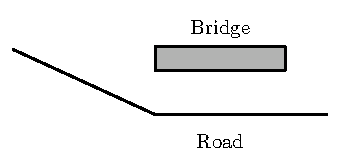
\includegraphics[width=.75\linewidth]{../figures/fhsm_2009_p64_f1.pdf}
      \end{center}

    \textbf{In the Classroom (Second-Year Mathematics)}

    In a visual model, one set of trailer wheels is jacked up on the sloping part of the road as the truck passes under the edge of the bridge. This position causes a portion of the trailer to be raised higher than it would be on a flat surface. The real question is, How much higher? The model that students construct likely will include characteristics similar to the model in the diagram at the right. Such a model should at least contain the line segment $PQ$---representing the ``dangerous height'' at which the trailer might hit the bridge. The model pictured here contains simplifying assumptions, such as representation of the wheels as circles and representation of the road as two straight line segments. Each simplifying assumption deserves discussion in class. In addition, after a fruitful discussion, the class may decide to measure the road grade in terms of degrees rather than as a percent. This decision is enacted in the analysis that follows. Some research by students may suggest that for most roadways, the road grade can reasonably be limited to what appears to be a small measure. In the present model, the road grade, $g$, is limited to $7$ degrees---at least in this iteration of the modeling cycle. (Although a grade angle of 7 degrees may be steep for a large truck, some diagrams here include a much larger grade angle to illuminate detail.)

      \begin{center}
        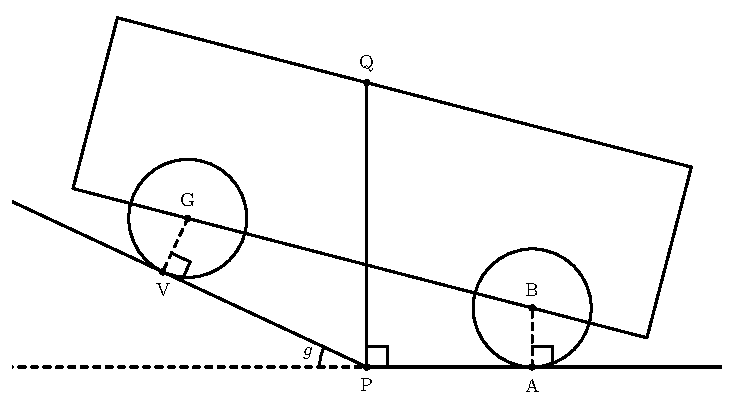
\includegraphics[width=.92\linewidth]{../figures/fhsm_2009_p64_2.pdf}
      \end{center}

    After students work on the construction of a model, an interactive computer model can be given to students so that they can explore how changes in various trailer dimensions and positions can affect the dangerous height, $PQ$. One of these variables is the distance the trailer is under the bridge. Another, more subtle variable is the distance between the wheel axles. (By itself, the overhang of the trailer beyond either wheel axle does not affect the dangerous height and can be ignored.) \vspace{\baselineskip}

    The next decision made by this class was to simplify the model even further during the first trip through the modeling cycle, taking the wheels off the truck. See the simplified model at the right. (The supporting topic book on geometry offers an analysis of the situation that uses the full model with the wheels on.)

      \begin{center}
        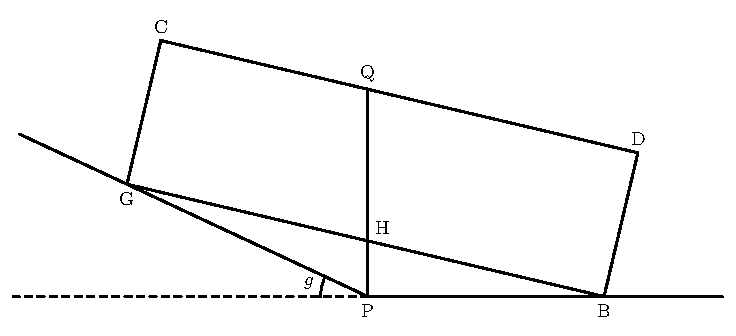
\includegraphics[width=.92\linewidth]{../figures/fhsm_2009_p65_1.pdf}
      \end{center}

    \textbf{Task 2}

    Task 2 asks the students to examine what might be lost or misrepresented by this simplification. We do not provide a detailed classroom discussion of task 2. However, students should realize that taking the wheels off and lowering the shortened trailer box does not simply lower the dangerous height by an amount equal to the wheel radius. Rather, the left (raised) end of the truncated trailer box is lowered a bit more than the right end, and this positioning does have an additional measurable effect on the dangerous height. Nevertheless, an analysis of the simplified model will help us analyze the original situation with the more complex model, in which the trailer has wheels. Moreover, even in this simpler case with a small grade angle, the result may be surprising.

    Tasks 3 and 4 ask students to explore relationships in the simplified model both geometrically and symbolically. 

    \textbf{Task 3}

    Let $d$ represent the length of segment $PQ$, $w$ represent the measure of angle $PBH$ (the tilt of the trailer), $s$ represent the length of segment $PB$ (how far the trailer is under the bridge), and $g$ represent the grade in degrees. Explore the situation by using your interactive drawing of the simplified model. See if you can get a feel for---or make a conjecture about---when the dangerous height, $d$, would be highest by considering $w$ or $s$ or both.

      \begin{center}
        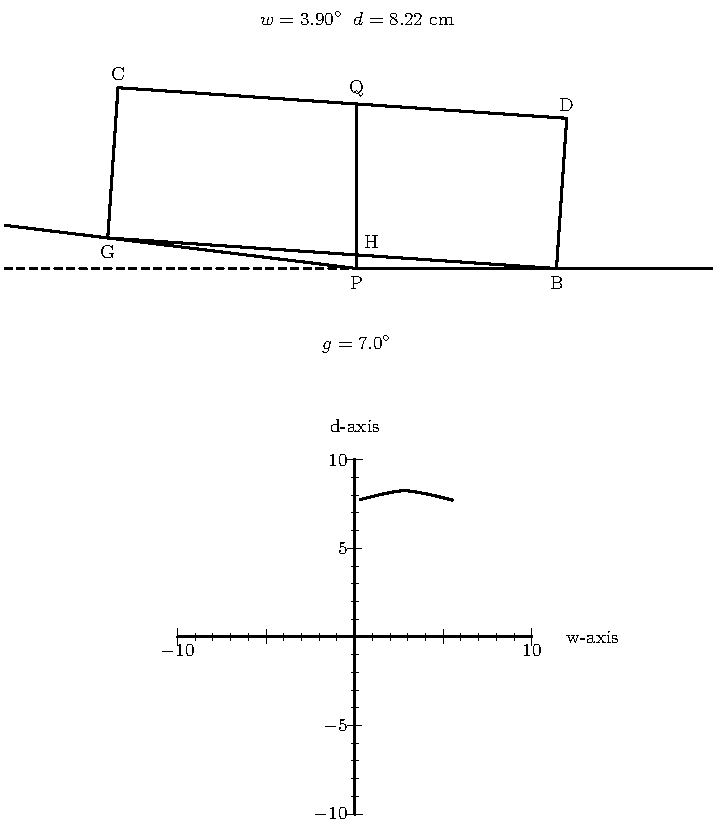
\includegraphics[width=.92\linewidth]{../figures/fhsm_2009_p66_f1.pdf}
      \end{center}

    \textbf{In the Classroom (Second-Year Mathematics)}

    One group used the interactive drawing to trace the graph of the dangerous height, $d$, as a function of $w$, as seen in the figure above, where they have set $g$ equal to $7$ degrees. They noted that they were not able to find a symbolic representation of this function but that it did suggest useful information. In their exploration, they used several small values of $g$, and each time the dangerous height looked greatest when\vspace{.5\baselineskip}
    $$
      w=\frac{g}{2}.
    $$

    Another group used large angles for grades, for instance, 55 degrees, and that pattern did not hold up. But other students raised the objection that such large grades were unrealistic and not within bounds of the model. More insight was sought about what happens for small values of $g$.

    After additional work, group 3 presented some theoretical evidence that adds some insight and support to the claim that the maximum value of the dangerous height occurs when
    $$
      w=\frac{g}{2}
    $$
    for the (small) values of $g$ that our model allows.

    Group 3 drew an analogy to example 15, ``Circling the Points,'' and envisioned $\angle GPB$ inscribed in a circle together with chord $GB$. The first thing to note is that the point $P$ changes position along the arc of the circle as the trailer box is drawn along the roadway. The perpendicular distance from $P$ to the chord $GB$ is greatest when the foot of this perpendicular, $K$, is the midpoint of segment $GB$.

      \begin{center}
        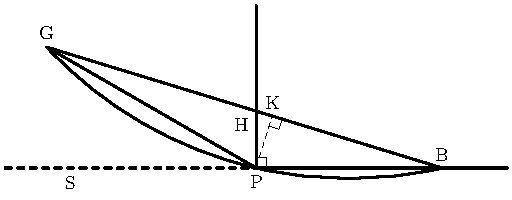
\includegraphics[width=.92\linewidth]{../figures/fhsm_2009_p66_f2.pdf}
      \end{center}

    \begin{scriptlist}
      \item [Student 3:] When $K$ is the midpoint of segment $GB$, angles $\angle PGB$ and $\angle PBG$ are congruent. I know that $m\angle PGB + m\angle PBG = m\angle SPG$, and the measure of angle $\angle SPG = g$. So now I have that
      $$
        m\angle PGB=m\angle PBG=\frac{g}{2}=w.
      $$

      Now I want to show that the part of the dangerous height represented by segment $PH$ is really close in length to segment $PK$---wherever $K$ is on $BG$. That is because the angle between segment $PK$ and segment $PH$ is small if $g$ is small. Here's why that is true. Triangles $PHK$ and $PHB$ are similar because they are right triangles that share $\angle PHK$. So $m\angle HPK = m\angle PBH = w$. But I know that $0 \leq w \leq g \leq 7^\circ$. Then $0.99 \leq \cos(w) \leq 1$. Since
      $$
        \cos(w)-\cos(\angle PHK)=\frac{\lvert PK\rvert}{\lvert PH\rvert},
      $$
      we've got that
      $$
        0.99\leq \frac{\lvert PK\rvert}{\lvert PH\rvert}\leq 1.
      $$

      This means the two lengths in the fraction are really, really close. \emph{The point is that part of the dangerous height represented by segment $PH$ should be maximized when the length of segment $PK$ is maximized, and that is when}
      $$
        m\angle PBG=\frac{g}{2}.
      $$

      \item [Teacher:] That gives some pretty solid support for the idea that there is at least a portion of the dangerous height that is at least close to being maximized when
      $$
        w=\frac{g}{2}.
      $$

      Let's continue by analyzing $d$ a little further.
    \end{scriptlist}

    \textbf{Task 4}

    Can you find a symbolic relationship between the tilt of the trailer, $w$, and the measure of the dangerous height $d$? You may use other measurements related to the model, such as $s$ (the distance the trailer is under the bridge, measured by segment $PB$), the length of the shortened trailer box (measured by segment $GB$), or some other measurement related to the situation. You may continue to find trigonometry useful.

    \textbf{In the Classroom (After Further Discussion)}

    \begin{scriptlist}
      \item [Group 5:] We did find trigonometry helpful. We found a relationship between the length of segment $PH$ and $w$ first. We got that
      $$
        \tan(w)=\frac{\lvert PH\rvert}{\lvert PB\rvert}.
      $$

      So $\lvert PB\rvert\tan(w)=\lvert PH\rvert$. That is, $s\cdot \tan(w)=\lvert PH\rvert$.

      \begin{center}
        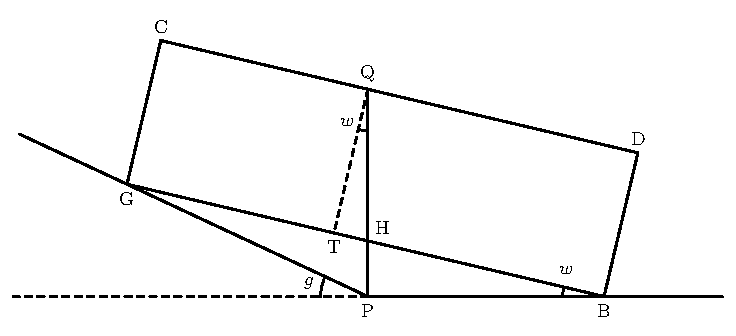
\includegraphics[width=.92\linewidth]{../figures/fhsm_2009_p68_1.pdf}
      \end{center}

      We wanted to find out something about the length of segment $HQ$ next. We didn't get anywhere at first, but then one of our group members noticed that this segment sort of replaces the original height of the truck. So we decided to compare it to the original height of the truck. So then we drew segment $QT$ perpendicular to $GB$. The length of segment $QT$ would be the original height of the truck. After we drew the segment, we saw that $\angle PHB$ and $\angle THQ$ were congruent because they are vertical angles. That makes the right triangles $PHB$ and $THQ$ similar. So $\angle HQT = w$. We let $h$ stand for the original height of the truck. That is, $h =\lvert QT\rvert$. So
      $$
        \cos(w)=\frac{h}{\lvert HQ\rvert}.
      $$

      This means that
      $$
        \lvert HQ\rvert=\frac{h}{\cos(w)}.
      $$

      We put these together and got\vspace{1.5\baselineskip}

      $$
        d=s\cdot \tan(w)+\frac{h}{\cos(w)}.
      $$

      \item [Teacher:] Good. That relationship works for any value of $w$ that occurs within the model. Now it is time to think about interpreting these results in the real world. What value of $g$ should we use in our formula?
      
      \item [Class:] Seven degrees.
      
      \item [Teacher:] We have gathered support for testing $w$ at
      $$
        \frac{g}{2},
      $$
      or $3.5$ degrees. For homework, research a good height to use for the trailer box and a good length for the trailer length between points $G$ and $B$. In addition, for
      $$
        w=\frac{g}{2}
      $$
      and $\lvert GB\rvert = m$, determine how one could figure out the value of $s$. We will need to do that to determine the value of $d$.\vspace{.5\baselineskip}
    \end{scriptlist}

    The next day students decide on $h = 10$ feet and $m = 40$ feet. In addition, $\triangle PGB$ is isosceles when
    $$
      w=\frac{g}{2}.
    $$

    By constructing the altitude from $P$ to side $GB$, one can derive the relationship
    $$
      \cos\left(\frac{g}{2}\right)=\frac{m/2}{s} \, \text{or} \, s=\frac{m/2}{\cos(g/2)}.
    $$

    With these values,
    $$
      d=\frac{20}{\cos(3.5)}\tan(3.5)+\frac{10}{\cos(3.5)}\approx 11.24 \, \text{feet},
    $$
    or about $11$ feet $3$ inches. Just looking at the value $7$ degrees as a small number might suggest that road grade does not matter. But our analysis for this specific and realistic example shows that with an initial trailer height of $10$ feet, the dangerous height for the trailer is \emph{at least a foot higher}! As Dr. Pollak noted, road grade cannot be ignored.\vspace{\baselineskip}

    \textbf{Key Elements of Mathematics}

    \begin{hanglist}
      \hangitem{Reasoning with Geometry---Geometric connections and modeling; Construction and evaluation of geometric arguments}
      \hangitem{Reasoning with Algebraic Symbols---Meaningful use of symbols; Mindful manipulation}
      \hangitem{Reasoning with Functions---Using multiple representations of functions}
    \end{hanglist}

    \textbf{Reasoning Habits}

    \begin{hanglist}
      \hangitem{Analyzing the problem---identifying relevant variables and conditions; seeking patterns and relationships; looking for hidden structure; considering special cases or simpler analogs}
      \hangitem{Implementing a strategy---making purposeful use of procedures; making logical deductions; monitoring progress toward a solution}
      \hangitem{Seeking and using connections}
      \hangitem{Reflecting on a solution---considering the reasonableness of a solution; justifying or validating a solution; reconciling different approaches; generalizing a solution}
    \end{hanglist}
  }
  {
    Chui cầu
  }
  {
    \textbf{Nhiệm vụ 1}

    Nhà toán học Henry Pollak (2004) từng suy nghĩ về việc vì sao tổ hợp xe đầu kéo thường bị mắc kẹt dưới gầm cầu, trong khi ``chiều cao tĩnh không tối đa'' đã được ghi rõ trên biển báo chiều cao của cầu. Cầu đang xét nằm ngang và ở ngay chân một đoạn đường dốc xuống. Trong nhiệm vụ khởi đầu này, học sinh được yêu cầu xây dựng mô hình trực quan hai chiều cho tình huống, đồng thời liệt kê giả thiết mà các em đưa ra.

    \begin{center}
      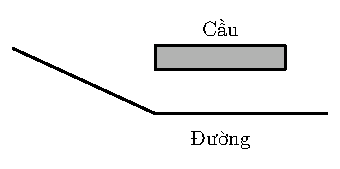
\includegraphics[width=.75\linewidth]{../figures/fhsm_2009_p64_f1_vi.pdf}
    \end{center}

    \textbf{Trong lớp học (toán năm thứ hai)}\vspace{\baselineskip}

    Trong mô hình trực quan, bộ bánh xe được nâng lên trên phần đường dốc khi xe đi qua dưới mép cầu. Vị trí này khiến một phần của toa hàng cao hơn so với khi xe ở trên mặt đường phẳng. Câu hỏi thật sự là: cao hơn bao nhiêu? Mô hình mà học sinh xây dựng nhiều khả năng sẽ có đặc điểm tương tự mô hình trong hình vẽ bên dưới. Mô hình như vậy tối thiểu phải chứa đoạn thẳng $PQ$---biểu thị ``độ cao nguy hiểm'' tại đó toa hàng có thể chạm vào cầu. Mô hình minh họa ở đây gồm những giả thiết đơn giản hóa, chẳng hạn biểu diễn bánh xe bằng đường tròn và biểu diễn mặt đường bằng hai đoạn thẳng. Mỗi giả thiết đơn giản hóa đều đáng được thảo luận trong lớp. Ngoài ra, sau cuộc thảo luận hiệu quả, lớp có thể quyết định đo độ dốc của đường theo độ thay vì theo phần trăm. Quyết định này được dùng trong phần phân tích tiếp theo. Một số tìm hiểu của học sinh có thể gợi ý rằng đối với hầu hết tuyến đường, độ dốc có thể được giới hạn hợp lí trong một khoảng nhỏ. Trong mô hình hiện tại, độ dốc của đường, $g$, được giới hạn đến 7 độ---ít nhất là trong vòng lặp này của chu trình mô hình hóa. (Mặc dù độ dốc 7 độ có thể khá lớn đối với một xe tải lớn, các hình vẽ ở đây dùng góc dốc lớn hơn nhiều để làm nổi bật chi tiết.)\vspace{3\baselineskip}

    \begin{center}
      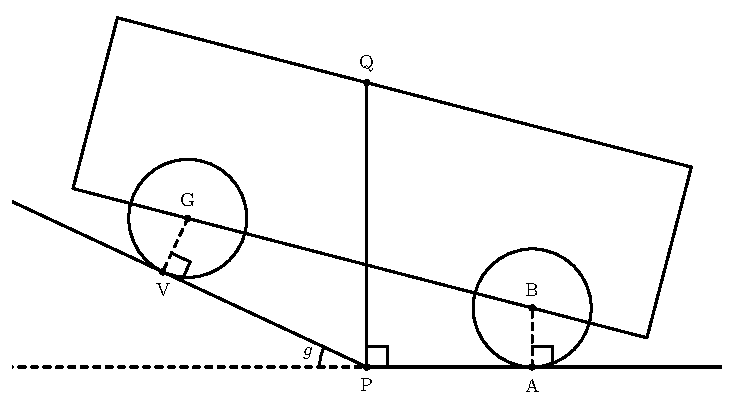
\includegraphics[width=.92\linewidth]{../figures/fhsm_2009_p64_2.pdf}
    \end{center}

    Sau khi học sinh hoàn thành việc xây dựng mô hình, có thể cung cấp cho các em mô hình máy tính tương tác để khám phá việc thay đổi kích thước và vị trí khác nhau của toa hàng ảnh hưởng thế nào đến độ cao nguy hiểm $PQ$. Một trong các biến số là khoảng cách mà toa hàng đã đi vào dưới gầm cầu. Một biến số khác, tinh tế hơn, là khoảng cách giữa hai trục bánh xe. (Tự thân phần toa hàng nhô ra vượt quá mỗi trục bánh xe không ảnh hưởng đến độ cao nguy hiểm và có thể bỏ qua.)\vspace{1\baselineskip}

    Quyết định tiếp theo của lớp là đơn giản hóa mô hình hơn nữa trong lượt đầu của chu trình mô hình hóa, bằng cách bỏ bánh xe khỏi xe. Xem mô hình đã đơn giản hóa ở hình bên dưới. (Sách chủ đề bổ trợ về hình học cung cấp phân tích tình huống này bằng mô hình đầy đủ có bánh xe.)

    \begin{center}
      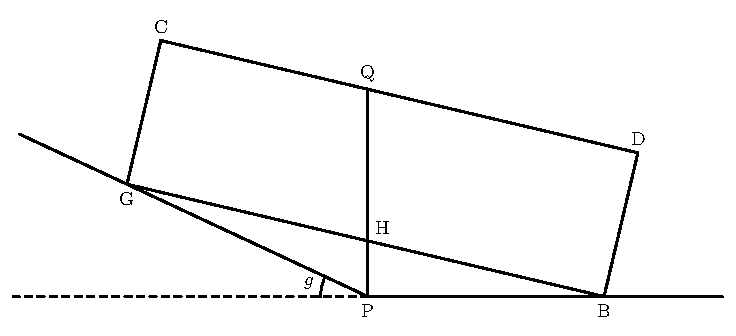
\includegraphics[width=.92\linewidth]{../figures/fhsm_2009_p65_1.pdf}
    \end{center}
    
    \textbf{Nhiệm vụ 2}

    Nhiệm vụ 2 yêu cầu học sinh xem xét những gì bị mất đi hoặc bị biểu diễn sai lệch do sự đơn giản hóa này. Ta không trình bày chi tiết phần thảo luận trên lớp cho Nhiệm vụ 2. Tuy nhiên, học sinh cần nhận thấy việc tháo bánh xe và hạ thấp toa hàng không đơn giản là làm giảm chiều cao nguy hiểm đi một lượng đúng bằng bán kính bánh xe. Đúng hơn, đầu bên trái (cao hơn) của toa hàng được hạ xuống nhỉnh hơn đầu bên phải; và chính tư thế này tạo thêm ảnh hưởng đo được đối với chiều cao nguy hiểm. Dù vậy, việc phân tích mô hình đơn giản hóa sẽ giúp ta xử lí tình huống ban đầu với mô hình phức tạp hơn, trong trường hợp toa hàng có bánh xe. Hơn nữa, ngay cả trong trường hợp đơn giản này, với góc dốc nhỏ, kết quả thu được vẫn có thể gây bất ngờ.\vspace*{\baselineskip}

    Nhiệm vụ 3 và 4 yêu cầu học sinh khám phá các quan hệ trong mô hình đơn giản hóa, cả bằng hình học lẫn bằng kí hiệu.

    \textbf{Nhiệm vụ 3}

    Gọi $d$ là độ dài đoạn $PQ$, $w$ là số đo góc $PBH$ (độ nghiêng của toa hàng), $s$ là độ dài đoạn $PB$ (mức độ toa hàng đã đi vào dưới gầm cầu), và $g$ là độ dốc tính theo độ. Hãy khảo sát tình huống bằng bản vẽ tương tác của mô hình đơn giản hóa. Hãy xem em có thể hình dung được---hoặc đưa ra phỏng đoán về---khi nào độ cao nguy hiểm $d$ đạt lớn nhất bằng cách xét $w$, hoặc $s$, hoặc cả hai.\vspace{\baselineskip}

      \begin{center}
        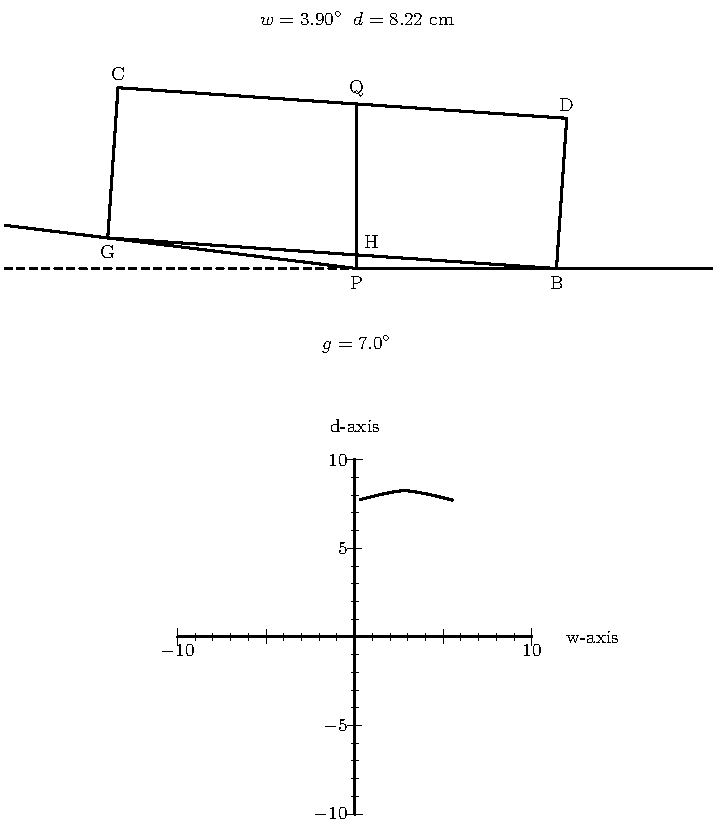
\includegraphics[width=.92\linewidth]{../figures/fhsm_2009_p66_f1_v2.pdf}
      \end{center}

    \textbf{Trong lớp học (toán năm thứ hai)} \vspace{\baselineskip}

    Một nhóm dùng hình vẽ tương tác để lần theo đồ thị của chiều cao nguy hiểm $d$ như một hàm theo $w$, như trong hình phía trên, trong đó các em đặt $g$ bằng 7 độ. Các em ghi nhận rằng mình chưa tìm được biểu diễn kí hiệu cho hàm số này, nhưng đồ thị vẫn gợi ra thông tin hữu ích. Trong quá trình khảo sát, các em thử vài giá trị nhỏ của $g$; mỗi lần như vậy, chiều cao nguy hiểm đều có vẻ đạt giá trị lớn nhất khi
    $$
      w=\frac{g}{2}.
    $$

    Một nhóm khác dùng các góc dốc lớn, chẳng hạn 55 độ, và mẫu hình ấy không còn đứng vững. Nhưng học sinh khác phản biện rằng những độ dốc lớn như vậy là phi thực tế và không nằm trong phạm vi của mô hình. Vì thế, lớp cần tìm hiểu thêm điều xảy ra với các giá trị nhỏ của $g$.

    Sau khi tiếp tục làm việc, Nhóm 3 trình bày một số bằng chứng lí thuyết, bổ sung sự hiểu và hỗ trợ cho nhận định rằng giá trị lớn nhất của độ cao nguy hiểm xảy ra khi
    $$
      w=\frac{g}{2}
    $$
    đối với các giá trị nhỏ của $g$ mà mô hình của chúng ta cho phép.

    Nhóm 3 liên hệ với Ví dụ 15, ``Đường tròn qua các điểm'', và hình dung rằng góc $\angle GPB$ là góc nội tiếp trong một đường tròn có dây cung $GB$. Điều đầu tiên cần lưu ý là điểm $P$ thay đổi vị trí dọc theo cung tròn khi toa hàng được kéo dọc theo mặt đường. Khoảng cách vuông góc từ $P$ đến dây cung $GB$ đạt lớn nhất khi chân đường vuông góc này, $K$, là trung điểm của đoạn $GB$.\vspace{\baselineskip}

    \begin{center}
      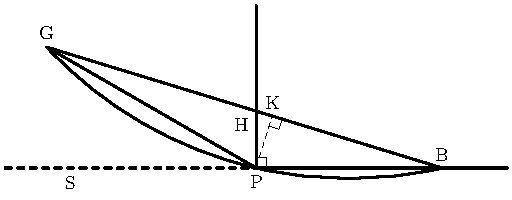
\includegraphics[width=.92\linewidth]{../figures/fhsm_2009_p66_f2.pdf}
    \end{center}

    \begin{scriptlist}
      \item [Học sinh 3:] Khi $K$ là trung điểm của đoạn $GB$, hai góc $\angle PGB$ và $\angle PBG$ bằng nhau. Em biết rằng $m\angle PGB + m\angle PBG = m\angle SPG$, và số đo của góc $\angle SPG$ bằng $g$. Vậy hiện giờ em có
      
      $$
        m\angle PGB=m\angle PBG=\frac{g}{2}=w.
      $$

      Bây giờ em muốn chỉ ra rằng phần độ cao nguy hiểm được biểu diễn bởi đoạn $PH$ có độ dài rất gần với đoạn $PK$---với mọi vị trí của $K$ trên $BG$. Đó là vì góc giữa đoạn $PK$ và đoạn $PH$ nhỏ nếu $g$ nhỏ. Lí do là như sau. Hai tam giác $PHK$ và $PHB$ đồng dạng vì chúng là các tam giác vuông và có chung một góc nhọn. Do đó $m\angle HPK = m\angle PBH = w$. Mà em biết $0^\circ \leq w \leq g \leq 7^\circ$. Khi đó $0.99 \leq \cos(w) \leq 1$. Vì
      $$
        \cos(w)-\cos(\angle PHK)=\frac{\lvert PK\rvert}{\lvert PH\rvert},
      $$
      nên ta có
      $$
        0.99\leq \frac{\lvert PK\rvert}{\lvert PH\rvert}\leq 1.
      $$

      Điều này có nghĩa là hai độ dài trong phân số rất gần nhau. \emph{Điểm mấu chốt là phần độ cao nguy hiểm được biểu diễn bởi đoạn $PH$ sẽ đạt giá trị lớn nhất khi độ dài đoạn $PK$ đạt giá trị lớn nhất, và điều đó xảy ra khi}\vspace{\baselineskip}

      $$
        m\angle PBG=\frac{g}{2}.
      $$

      \item [Giáo viên:] Điều đó cung cấp cơ sở khá vững chắc cho ý tưởng rằng ít nhất một thành phần của chiều cao nguy hiểm gần đạt giá trị lớn nhất khi

      $$
        w=\frac{g}{2}.
      $$

      Ta hãy tiếp tục bằng việc phân tích $d$ thêm một chút.
    \end{scriptlist}

    \textbf{Nhiệm vụ 4}

    Em có thể tìm quan hệ bằng kí hiệu giữa độ nghiêng của toa hàng, $w$, và độ cao nguy hiểm $d$ không? Em có thể dùng đại lượng khác liên quan đến mô hình, chẳng hạn $s$ (khoảng cách toa hàng đã đi vào dưới gầm cầu, đo bởi đoạn $PB$), độ dài toa hàng đã rút ngắn (đo bởi đoạn $GB$), hoặc đại lượng khác liên quan đến tình huống. Lượng giác có thể tiếp tục hữu ích. \vspace{2\baselineskip}

    \textbf{Trong lớp học (sau khi thảo luận thêm)} \vspace{\baselineskip}

    \begin{scriptlist}
      \item [Nhóm 5:] Chúng em thấy lượng giác hữu ích. Trước hết, chúng em tìm được quan hệ giữa độ dài đoạn $PH$ và $w$. Chúng em có
      $$
        \tan(w)=\frac{\lvert PH\rvert}{\lvert PB\rvert}.
      $$

      Vậy $\lvert PB\rvert\tan(w)=\lvert PH\rvert$. Tức là, $s\cdot \tan(w)=\lvert PH\rvert$.
      
      \begin{center}
        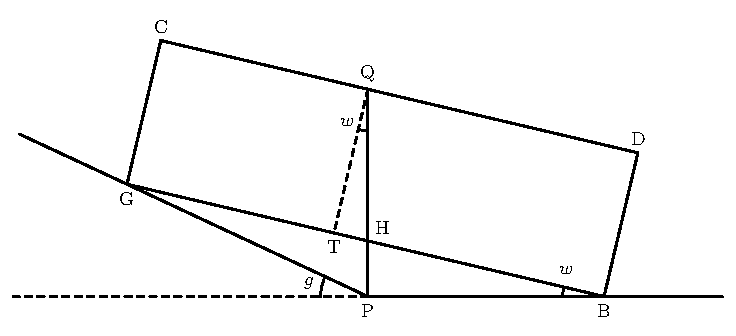
\includegraphics[width=.92\linewidth]{../figures/fhsm_2009_p68_1.pdf}
      \end{center}

      Tiếp theo, chúng em muốn tìm hiểu độ dài đoạn $HQ$. Lúc đầu chúng em không đi đến đâu, nhưng rồi một bạn trong nhóm nhận ra rằng đoạn này gần như thay cho chiều cao ban đầu của xe. Vì vậy, chúng em quyết định so sánh nó với chiều cao ban đầu của xe. Chúng em kẻ đoạn $QT$ vuông góc với $GB$. Độ dài đoạn $QT$ sẽ là chiều cao ban đầu của xe. Sau khi kẻ đoạn này, chúng em thấy $\angle PHB$ và $\angle THQ$ bằng nhau vì chúng là hai góc đối đỉnh. Do đó hai tam giác vuông $PHB$ và $THQ$ đồng dạng. Suy ra $\angle HQT=w$. Chúng em kí hiệu $h$ là chiều cao ban đầu của xe, tức là $h=\lvert QT\rvert$. Khi đó\vspace{2\baselineskip}

      $$
        \cos(w)=\frac{h}{\lvert HQ\rvert}.
      $$

      Điều này cho thấy
      $$
        \lvert HQ\rvert=\frac{h}{\cos(w)}.
      $$

      Ghép các kết quả lại, chúng em được
      $$
        d=s\cdot \tan(w)+\frac{h}{\cos(w)}.
      $$

      \item [Giáo viên:] Tốt. Quan hệ đó đúng với mọi giá trị của $w$ xuất hiện trong mô hình. Bây giờ đã đến lúc nghĩ về việc diễn giải các kết quả này trong thế giới thực. Trong công thức của chúng ta, nên dùng giá trị nào cho $g$?
      
      \item [Cả lớp:] Bảy độ.
      
      \item [Giáo viên:] Chúng ta đã có cơ sở để thử $w$ tại
      $$
        \frac{g}{2},\vspace{\baselineskip}
      $$
      tức $3.5$ độ. Về nhà, hãy tìm hiểu chiều cao hợp lí để dùng cho toa hàng và độ dài hợp lí cho phần chiều dài toa hàng giữa các điểm $G$ và $B$. Ngoài ra, với
      $$
        w=\frac{g}{2}
      $$
      và $\lvert GB\rvert = m$, hãy xác định cách ta có thể tìm ra giá trị $s$. Chúng ta sẽ cần điều đó để xác định giá trị $d$.
    \end{scriptlist}

    Ngày hôm sau, học sinh chọn $h = 10$ foot\footnote{Foot (ft): đơn vị đo chiều dài trong hệ Mỹ; $1\;\text{foot}=12\;\text{inch}=0{,}3048\;\text{m}$.} và $m = 40$ foot. Ngoài ra, tam giác $\triangle PGB$ cân khi
    $$
      w=\frac{g}{2}.
    $$

    Bằng cách dựng đường cao từ $P$ xuống cạnh $GB$, ta suy ra hệ thức
    $$
      \cos\left(\frac{g}{2}\right)=\frac{m/2}{s} \; \text{hoặc} \; s=\frac{m/2}{\cos(g/2)}.
    $$

    Với các giá trị này,
    $$
      d=\frac{20}{\cos(3.5)}\tan(3.5)+\frac{10}{\cos(3.5)}\approx 11.24 \; \text{foot},
    $$
    tức khoảng 11 foot thêm 3 inch. Chỉ nhìn 7 độ như một số nhỏ có thể khiến người ta nghĩ rằng độ dốc của con đường không đáng kể. Nhưng phân tích của chúng ta trong ví dụ cụ thể và thực tế này cho thấy: với chiều cao ban đầu của toa hàng là 10 foot, độ cao nguy hiểm đối với toa hàng \emph{ít nhất cao hơn 1 foot}! Như Dr. Pollak đã nhận xét, độ dốc của con đường không thể bị bỏ qua.

    \textbf{Các yếu tố then chốt của toán học}

    \begin{hanglist}
      \hangitem{Luận với hình học---Các kết nối hình học và mô hình hóa; Xây dựng và thẩm định các lập luận hình học}

      \hangitem{Luận với kí hiệu đại số---Sử dụng kí hiệu có nghĩa; Biến đổi có ý thức}\vspace{\baselineskip}

      \hangitem{Luận với hàm số---Sử dụng nhiều biểu diễn của hàm số}
    \end{hanglist}

    \textbf{Thói quen luận}

    \begin{hanglist}
      \hangitem{Phân tích bài toán---xác định cẩn thận biến và điều kiện thích đáng; tìm kiếm mẫu hình và quan hệ; tìm kiếm cấu trúc ẩn; xét trường hợp đặc biệt hoặc dạng tương tự đơn giản hơn}

      \hangitem{Triển khai chiến lược---vận dụng thủ tục có chủ đích; thực hiện suy diễn logic; theo dõi tiến trình đi đến lời giải}\vspace{\baselineskip}

      \hangitem{Tìm kiếm và sử dụng kết nối}

      \hangitem{Phản tư về lời giải---xem xét tính hợp lí của lời giải; biện minh hoặc kiểm chứng lời giải; dung hòa những cách tiếp cận khác nhau; khái quát hóa lời giải}
    \end{hanglist}
  }
  {
    Công thức $\cos(w)-\cos(\angle PHK)=\frac{\lvert PK\rvert}{\lvert PH\rvert}$ được giữ theo bản gốc. Tuy nhiên, xét theo lập luận ngay trước đó, vì $m\angle HPK=w$ trong tam giác $PHK$, hệ thức tự nhiên về mặt lượng giác phải là $\cos(w)=\frac{\lvert PK\rvert}{\lvert PH\rvert}$. Do đó, công thức trong bản gốc có khả năng là lỗi chế bản hoặc lỗi nhận dạng kí tự.
  }

\TriPara
  {
    \EN{The geometry strand extends beyond two- and three-dimensional figures in Euclidean space to include other special configurations and visualizations. Example 18 illustrates a modeling context in which the most obvious geometric model of the situation---drawing circles of radius $5$ units and looking for overlaps that represent radio interference---is not the most useful. Rather, a basic representation in the growing fi eld of ``graph theory''---usually considered a domain within discrete mathematics---is better suited to capture the relevant information in the modeling problem.}
  }
  {
    \VI{Mạch hình học không chỉ giới hạn ở các hình hai chiều và ba chiều trong không gian Euclid, mà còn bao gồm những cấu hình đặc biệt và cách hình dung trực quan đặc biệt khác. Ví dụ 18 minh họa một bối cảnh mô hình hóa trong đó mô hình hình học dễ thấy nhất của tình huống---vẽ các đường tròn bán kính 5 đơn vị và tìm vùng chồng lấn biểu thị nhiễu sóng vô tuyến---lại không phải là mô hình hữu ích nhất. Thay vào đó, một cách biểu diễn cơ bản trong lĩnh vực đang phát triển của ``lí thuyết đồ thị''---thường được xem là một lĩnh vực thuộc toán học rời rạc---phù hợp hơn để nắm bắt thông tin liên quan trong bài toán mô hình hóa.}
  }{\NOTE{}}

\TriExample
  {
    Assigning Frequencies
  }
  {
    \textbf{Task}

    The Federal Communications Commission (FCC) needs to assign radio frequencies to seven new radio stations located on the grid at the right. Such assignments are based on several considerations, including the possibility of creating interference by assigning the same frequency to stations that are too close together. In this simplified situation, we assume that broadcasts from two stations located within $200$ miles of each other will create interference if they broadcast on the same frequency, whereas stations more than $200$ miles apart can use the same frequency to broadcast without causing interference with each other.

    \begin{center}
      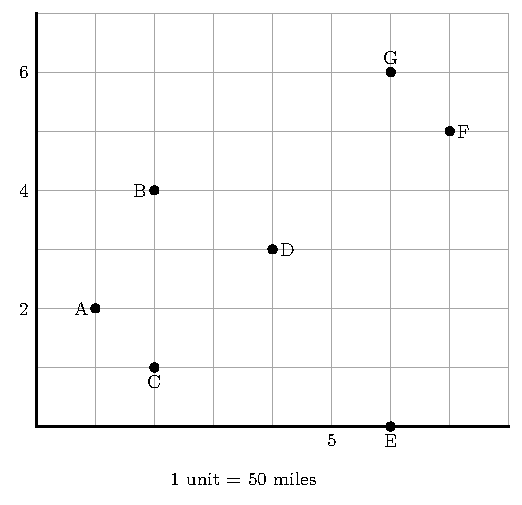
\includegraphics[width=.92\linewidth]{../figures/fhsm_2009_p70_f1.pdf}
    \end{center}

    How can a vertex-edge graph be used to assign frequencies so that the fewest number of frequencies are used and no stations interfere with each other? What would each vertex represent? What would an edge represent? What is the fewest number of frequencies needed? (Adapted from Hirsch et al. [2007])

    \textbf{In the Classroom}

    Students work on the task in groups. Each group seems to agree that a vertex in the graph represents a radio station. So the graph would have seven vertices. Some groups decide to make a graph model in which two vertices representing stations within 200 miles of each other will be joined by an edge.

    \begin{center}
      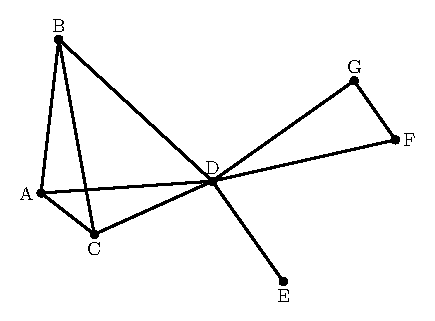
\includegraphics[width=.92\linewidth]{../figures/fhsm_2009_p71_1.pdf}
    \end{center}

    Other groups suggest that two vertices will be joined with an edge if they are \emph{more} than 200 miles apart. After some discussion, the choice is made to use the first suggestion, that of joining vertices with an edge if the distance between them is no more than 200 miles. The next task is to construct the model. Doing so requires computation of the distance between each pair of stations. Groups make these computations by using the distance formula or Pythagorean theorem and a calculator. Organization is valuable here because many computations are involved. Some groups might start by computing the distance from $A$ to the remaining six stations, then the distance from $B$ to the remaining five, and so on. A quick determination of how many computations are needed can help determine whether any list is missing an item. Experience with example 10, ``Patterns, Plane and Symbol,'' would be useful in this context.

    Groups produce models similar to the one above and then work at assigning frequencies to vertices so that no two vertices joined by a single edge have the same frequency. They look for a method that will use the fewest frequencies for this particular graph. One group explained their solution this way:

    ``We found that the fewest number of frequencies that could be used was four. We reasoned this way: First, look at the collection of vertices $A$ through $D$. Each of these vertices is joined by an edge to each of the other three in the collection. So no two vertices in the collection can have the same frequency. That means you can have no fewer than four frequencies.

    Next, suppose you assign frequency 1 to vertex $A$, frequency 2 to vertex $B$, frequency 3 to vertex $C$, and frequency 4 to vertex $D$. You can finish the assignment by assigning frequency 1 to vertex $G$ (because $G$ doesn't interfere with $A$), frequency 2 to vertex $F$, and frequency 3 to vertex $E$. That proves you don't need any more than four frequencies. That does it!''

    \textbf{Key Elements of Mathematics}

    \begin{hanglist}
      \hangitem{Reasoning with Geometry---Geometric connections and modeling; Construction of geometric arguments}
    \end{hanglist}

    \textbf{Reasoning Habits}

    \begin{hanglist}
      \hangitem{Analyzing a problem---seeking patterns and relationships; applying previously learned concepts}

      \hangitem{Implementing a strategy---organizing a solution; making logical deductions}

      \hangitem{Reflecting on a solution---justifying or validating a solution}
    \end{hanglist}
  }
  {
    Xếp tần số
  }
  {
    \textbf{Nhiệm vụ}

    Ủy ban Truyền thông Liên bang Hoa Kì (Federal Communications Commission---FCC) cần phân bổ tần số vô tuyến cho bảy đài phát thanh mới, được đặt tại các vị trí trên lưới tọa độ như trong hình bên dưới. Việc phân bổ này dựa trên nhiều yếu tố, trong đó có khả năng xảy ra nhiễu sóng khi gán cùng tần số cho các đài ở quá gần nhau. Trong tình huống đã được đơn giản hóa này, ta giả sử rằng các đài phát thanh cách nhau không quá $200$ mile\footnote{Mile (mi): Đơn vị đo chiều dài trong hệ Mỹ; $1\;\text{mi}=1.61\;\text{km}$} sẽ gây nhiễu nếu cùng phát trên một tần số, trong khi các đài cách nhau hơn $200$ mile có thể sử dụng cùng tần số mà không gây nhiễu cho nhau.\vspace{\baselineskip}

    \begin{center}
      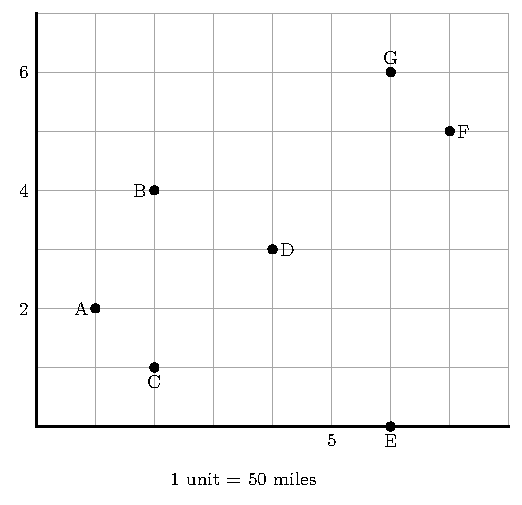
\includegraphics[width=.92\linewidth]{../figures/fhsm_2009_p70_f1.pdf}
    \end{center}

    Có thể sử dụng đồ thị đỉnh-cạnh như thế nào để gán tần số sao cho dùng ít tần số nhất và không có đài nào gây nhiễu cho nhau? Mỗi đỉnh sẽ biểu diễn gì? Mỗi cạnh sẽ biểu diễn gì? Số tần số ít nhất cần dùng là bao nhiêu? (Phỏng theo Hirsch et al. [2007])\vspace{\baselineskip}

    \textbf{Trong lớp học}

    Học sinh làm việc theo nhóm. Mỗi nhóm dường như đều đồng ý rằng một đỉnh trong đồ thị biểu diễn một đài phát thanh. Vì vậy, đồ thị sẽ có bảy đỉnh. Một số nhóm quyết định xây dựng mô hình đồ thị trong đó hai đỉnh biểu diễn hai đài cách nhau không quá $200$ mile sẽ được nối với nhau bằng một cạnh.

    \begin{center}
      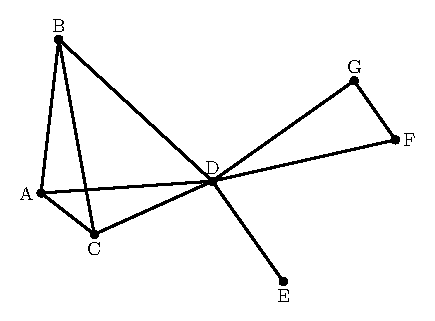
\includegraphics[width=.92\linewidth]{../figures/fhsm_2009_p71_1.pdf}
    \end{center}

    Một số nhóm khác đề xuất rằng hai đỉnh sẽ được nối với nhau bằng một cạnh nếu chúng cách nhau \emph{hơn} $200$ mile. Sau một hồi thảo luận, lớp quyết định chọn đề xuất thứ nhất: nối hai đỉnh bằng một cạnh nếu khoảng cách giữa hai đài tương ứng không quá $200$ mile. Nhiệm vụ tiếp theo là xây dựng mô hình. Việc này đòi hỏi phải tính khoảng cách giữa từng cặp đài. Các nhóm thực hiện những phép tính này bằng công thức khoảng cách hoặc định lí Pythagoras cùng với máy tính cầm tay. Việc tổ chức có giá trị ở đây, vì cần thực hiện khá nhiều phép tính. Một số nhóm có thể bắt đầu bằng cách tính khoảng cách từ $A$ đến sáu đài còn lại, rồi khoảng cách từ $B$ đến năm đài còn lại, và cứ tiếp tục như vậy. Việc xác định nhanh cần bao nhiêu phép tính có thể giúp kiểm tra xem danh sách có bị thiếu trường hợp nào hay không. Kinh nghiệm từ Ví dụ 10, ``Thêm đường thêm miền'', sẽ hữu ích trong bối cảnh này.

    Các nhóm tạo ra những mô hình tương tự như hình trên, rồi tiến hành gán tần số cho các đỉnh sao cho không có hai đỉnh nào được nối bởi một cạnh lại có cùng tần số. Các em tìm kiếm một phương pháp dùng ít tần số nhất cho đồ thị cụ thể này. Một nhóm trình bày lời giải của mình như sau:

    ``Chúng em nhận thấy số tần số ít nhất có thể dùng là bốn. Chúng em luận như sau: Trước hết, xét tập hợp các đỉnh từ $A$ đến $D$. Mỗi đỉnh trong tập hợp này đều được nối bằng một cạnh với ba đỉnh còn lại trong tập hợp. Vì vậy, không có hai đỉnh nào trong tập hợp này có thể có cùng tần số. Điều đó có nghĩa là không thể dùng ít hơn bốn tần số.\vspace{\baselineskip}

    Tiếp theo, giả sử ta gán tần số 1 cho đỉnh $A$, tần số 2 cho đỉnh $B$, tần số 3 cho đỉnh $C$, và tần số 4 cho đỉnh $D$. Ta có thể hoàn tất việc gán bằng cách gán tần số 1 cho đỉnh $G$ (vì $G$ không gây nhiễu với $A$), tần số 2 cho đỉnh $F$, và tần số 3 cho đỉnh $E$. Điều đó chứng tỏ ta không cần dùng nhiều hơn bốn tần số. Vậy là xong!''\vspace{\baselineskip}

    \textbf{Các yếu tố then chốt của toán học}

    \begin{hanglist}
      \hangitem{Luận với hình học---Các kết nối hình học và mô hình hóa; Xây dựng và thẩm định các lập luận hình học}
    \end{hanglist}

    \textbf{Thói quen luận}

    \begin{hanglist}
      \hangitem{Phân tích bài toán---tìm kiếm mẫu hình và quan hệ; vận dụng khái niệm đã học}\vspace{\baselineskip}

      \hangitem{Triển khai chiến lược---tổ chức lời giải; thực hiện những suy diễn logic}

      \hangitem{Phản tư về lời giải---biện minh hoặc kiểm chứng lời giải}
    \end{hanglist}
  }{}

\TriPara
  {
    \EN{Note that the vertex-edge representation of the frequency-assignment problem seems to have facilitated the structuring of an argument that four frequencies suffice---and even a way (algorithm) to assign four frequencies---for this example. Finding efficient algorithms for analogues of the general fewest-frequency problem for larger graphs remains an active area of current mathematical research. Such algorithms would find uses in many contexts.}
  }
  {
    \VI{Lưu ý rằng cách biểu diễn đỉnh-cạnh của bài toán gán tần số dường như đã giúp tổ chức lập luận rằng bốn tần số là đủ---và thậm chí còn gợi ra một cách làm (thuật toán) để gán bốn tần số---trong ví dụ này. Việc tìm thuật toán hiệu quả cho những bài toán tương tự bài toán tổng quát về số tần số ít nhất, trong trường hợp đồ thị lớn hơn, hiện vẫn là mảng nghiên cứu toán học đang tiếp diễn. Những thuật toán như vậy có thể được dùng trong nhiều bối cảnh.}
  }{\NOTE{}}

\TriPara
  {
    \EN{Geometry offers an inviting context in which students can develop their reasoning and sense making abilities. In addition, geometry provides tools and representations that are useful in a wide range of situations.}
  }
  {
    \VI{Hình học mang đến bối cảnh hấp dẫn để học sinh phát triển năng lực luận và hiểu. Bên cạnh đó, hình học còn cung cấp công cụ và cách biểu diễn hữu ích trong nhiều tình huống.}
  }{\NOTE{}}

\CloseGrid